\documentclass[11pt, letterpaper]{article}

\usepackage{mathptmx} % This is Times font
\usepackage[T1]{fontenc} % This is needed to get symbols like ~ correct
\usepackage{ifthen}
\usepackage{color}
\usepackage[hmarginratio=1:1,top=32mm]{geometry} % Document margins
\usepackage[hang, small,labelfont=bf,up,textfont=it,up]{caption} % Custom captions under/above floats in tables or figures
\usepackage{booktabs} % Horizontal rules in tables
\usepackage{float} % Required for tables and figures in the multi-column environment - they need to be placed in specific locations with the [H] (e.g. \begin{table}[H])
\usepackage{hyperref} % For hyperlinks in the PDF
\usepackage{graphicx}
\usepackage{subcaption}
\usepackage{enumitem}

\setlength{\parindent}{1em}
\setlength{\parskip}{1em}

\newcommand{\paragraphbe}[1]{\vspace{.75ex}\noindent{\textbf{\textit{ #1}}} }

\newboolean{publicversion}
\setboolean{publicversion}{false}
% \setboolean{publicversion}{true}

\ifthenelse{\boolean{publicversion}}{
	\newcommand{\grumbler}[3]{}
}{
	\newcommand{\grumbler}[3]{\textcolor{#3}{\bf #1: #2}}
}

% Add your own...
\newcommand{\aak}[1]{\grumbler{AA}{#1}{blue}}
\newcommand{\don}[1]{\grumbler{DP}{#1}{red}}
\newcommand{\cjr}[1]{\grumbler{CJR}{#1}{purple}}

\def\longconferencenames{}
% Conference macros
% include this in enclosing document for long conference names
%\def\longconferencenames{}

%  Use this one for the cv notes
%\def\includecvnotes{}
%\def\includebionotes{}

\newcommand{\conferencename}[3]{
\ifx\longconferencenames\undefined
\newcommand{#1}[0]{{#2}}
\else
\newcommand{#1}[0]{{#3}}
\fi
}

\newcommand{\cvnote}[1]{
\ifx\includecvnotes\undefined
%
\else
{#1}%
\fi
}


\newcommand{\bionote}[1]{
\ifx\includebionotes\undefined
%
\else
{#1}%
\fi
}


\conferencename{\podc}{PODC}{Proceedings of the ACM symposium on Principles of
distributed computing (PODC)}

\conferencename{\asplos}{ASPLOS}{{Proceedings of the ACM International Conference on Architectural Support for Programming Languages and Operating Systems (ASPLOS)}}

\conferencename{\spaa}{SPAA}{{Proceedings of the ACM symposium on Parallelism in algorithms and architectures (SPAA)}}

\conferencename{\osdi}{OSDI}{{Proceedings of the USENIX Symposium on Operating Systems Design and Implementation (OSDI)}}

\conferencename{\disc}{DISC}{{Proceedings of the International Conference on Distributed Computing (DISC)}}

\conferencename{\usenixatc}{USENIX ATC}{{Proceedings of the USENIX Annual Technical Conference}}
\conferencename{\usenixsec}{USENIX Security}{{Proceedings of the USENIX Security Symposium}}

\conferencename{\pldi}{PLDI}{{Proceedings of the ACM SIGPLAN conference on Programming language design and implementation (PLDI)}}

\conferencename{\computer}{Computer}{{IEEE Computer}}

\conferencename{\sosp}{SOSP}{{Proceedings of the ACM SIGOPS Symposium on Operating Systems Principles (SOSP)}}

\conferencename{\isca}{ISCA}{{Proceedings of the ACM IEEE International Symposium on Computer Architecture (ISCA)}}

\conferencename{\csaw}{CSAW}{{Proceedings of the ACM Workshop on Computer Security Architecture (CSAW)}}

\conferencename{\wddd}{WDDD}{{Proceedings of the Workshop on Duplicating, Deconstructing, and Debunking (WDDD)}}

\conferencename{\vldb}{VLDB}{{Proceedings of the International Conference on Very Large Databases (VLDB)}}

\conferencename{\toplas}{TOPLAS}{{ACM Transactions on Programming Languages and Systems (TOPLAS)}}

\conferencename{\tocs}{TOCS}{{ACM Transactions on Computer Systems (TOCS)}}

\conferencename{\ppopp}{{PPoPP}}{{Proceedings of the ACM SIGPLAN Symposium on Principles and Practice of Parallel Programming (PPoPP)}}

\conferencename{\jpdc}{J. Parallel Distrib. Comput.}{{Journal of Parallel and Distributed Computing}}

\conferencename{\ismm}{ISMM}{{Proceedings of the ACM International Symposium on Memory Management (ISMM)}}

\conferencename{\cacm}{CACM}{{Communications of the ACM (CACM)}}

\conferencename{\hpca}{HPCA}{{Proceedings of the IEEE International Symposium on High-Performance Computer Architecture (HPCA)}}

\conferencename{\transact}{TRANSACT}{{Proceedings of the ACM SIGPLAN Workshop on Transactional Computing (TRANSACT)}}

\conferencename{\iiswc}{IISWC}{{Proceedings of the IEEE International Symposium on Workload Characterization (IISWC)}}

\conferencename{\tpds}{IEEE Trans, Parallel Distrib. Syst.}{{IEEE Transactions on Parallel and Distributed Systems}}

\conferencename{\osr}{OSR}{{ACM Operating Systems Review}}

\conferencename{\nsdi}{NSDI}{{Proceedings of the USENIX Symposium on Networked Systems Design and Implementation (NSDI)}}

\conferencename{\cc}{CC}{{Proceedings of the International Conference on Compiler Construction (CC)}}

\conferencename{\surveys}{ACM Comput. Surv.}{{ACM Computing Surveys}}
\conferencename{\icde}{ICDE}{{Proceedings of the IEEE International Conference on Data Engineering (ICDE)}}
\conferencename{\fast}{FAST}{{Proceedings of the USENIX Conference on File and Storage Technologies (FAST)}}
\conferencename{\eurosys}{{E}uro{S}ys}{{Proceedings of the ACM European Conference on Computer Systems ({E}uro{S}ys)}}
\conferencename{\hotos}{HotOS}{{Proceedings of the USENIX Workshop on Hot Topics in Operating Systems (HotOS)}}
\conferencename{\hotcloud}{HotCloud}{{Proceedings of the USENIX Workshop on Hot Topics in Cloud Computing (HotCloud)}}
\conferencename{\oopsla}{OOPSLA}{{Proceedings of the ACM SIGPLAN Conference on Object-Oriented Programming, Systems, Languages, and Applications (OOPSLA)}}
\conferencename{\ndss}{NDSS}{{Proceedings of the Network and Distributed System Security Symposium (NDSS)}}
\conferencename{\oakland}{IEEE S\&P}{{Proceedings of the IEEE Symposium on Security and Privacy (Oakland)}}
\conferencename{\ispass}{ISPASS}{Proceedings of the IEEE International Symposium on Performance Analysis of Systems and Software (ISPASS)}

\conferencename{\europar}{{E}uro{P}ar}{{Proceedings of the European Conference on Parallel Programming ({E}uro{P}ar)}}

\conferencename{\sigcse}{{SIGCSE}}{{Proceedings of the ACM SIGCSE technical symposium on Computer science education (SIGCSE)}}

\conferencename{\ccs}{{CCS}}{{Proceedings of the ACM Conference on Computer and Communications Security (CCS)}}

\conferencename{\veeconf}{{VEE}}{{Proceedings of the International Conference on Virtual Execution Environments (VEE)}}

\conferencename{\lisa}{{LISA}}{{Proceedings of the Large Installation System Administration Conference (LISA)}}
\conferencename{\scool}{SCOOL}{{Proceedings of the Workshop on Synchronization and Concurrency in Object-Oriented Languages (SCOOL)}}
\conferencename{\cgo}{CGO}{{Proceedings of the International Symposium on Code Generation and Optimization (CGO)}}
\conferencename{\dsn}{{DSN}}{Proceedings of the International Conference on Dependable Systems and Networks (DSN)}
\conferencename{\sac}{{SAC}}{{Proceedings of the ACM Symposium on Applied Computing (SAC)}}

\conferencename{\cluster}{{IEEE Cluster}}{{IEEE International Conference on Cluster Computing}}


%------------------------------------------------------------------------------
%	TITLE SECTION
%------------------------------------------------------------------------------

\title{\vspace{-15mm}\huge\textbf{ Toward Efficient and Realizable Hardware Virtualization} \vspace{-5mm}}

\author{\large\textsc{Amogh Akshintala}}
\date{}

%------------------------------------------------------------------------------

\begin{document}

\maketitle % Insert title

% !TeX root = proposal.tex
\begin{abstract}
The proposed dissertation will focus on developer effort and compatibility in
software virtualization of CPU ISAs, and software virtualization of
specialized compute devices (e.g., GPUs, TPUs) that are programmed through an
API.

Although binary translation is a well-established software ISA virtualization
technique, given the size and complexity of today's dominant ISAs, developers
are routinely forced to adopt ad-hoc techniques to prioritize development
effort. The proposed dissertation will present a principled approach to
determine priority among different parts of the ISA. We believe this data will
be useful to designers of virtual ISAs as well.

Specialized compute accelerators, such as GPUs and TPUs, are usually
controlled through a user-space API.
The proposed dissertation will show that unlike with CPUs, where the ISA is
the canonical interface provided to the programmer, ISA virtualization is
untenable for specialized compute accelerators. Further, the proposed
dissertation will present a present a novel taxonomy, \emph{IEMTS} for cleanly
understanding the design space for virtualizing compute accelerators.
Based on insights from this taxonomy, the proposed dissertation will
present a novel virtualization technique, \emph{hypervisor-mediated
API-remoting}, that is at once realizable and performant.
\end{abstract}
% !TeX root = proposal.tex
\section{Introduction}
\label{sec:intro}

Virtualization has a long and tumultuous history. Virtual memory was first
described by German physicist Fritz-Rudolf Güntsch in his doctoral
dissertation in 1956~\cite{virtual-memory} and commercialized~\cite{atlas-vm}
in the Cambridge University/Ferranti Inc. Atlas computer. Virtually all
computers since then support virtual memory, with most providing hardware
units---\emph{Memory Management Unit (MMU)}---to accelerate the virtualization
of memory.

\emph{Hardware virtualization}~\cite{cp40}---the idea of virtualizing the
entire computer to enable the simultaneous execution of multiple Operating
Systems (OS)---was invented in 1962, and commercialized as the IBM
VM-370~\cite{vm370} hypervisor for the IBM 370 computer.
Virtualization was briefly forgotten through the 1980s and 1990s, as the
mainframe computer became all but obsolete during the Personal Computer (PC)
revolution. Intel's x86 Instruction Set Architecture (ISA), which came to
dominate the PCs that transplanted the mainframes, was not designed to be
traditionally virtualizable~\cite{popek-goldberg}, and was widely considered
unvirtualizable~\cite{gelsinger-pc,bugnion-workstation}. Multiple vendors
introduced \emph{software emulation} based solutions to enable the execution
of one OS on top of another (e.g., Insignia SoftPC, Connectix VirtualPC,
VMware Workstation). Over time, better techniques were devised to virtualize
the x86 ISA, including ISA extensions (e.g., AMD-V and Intel VT-x) to enable
native execution of virtualized applications, only trapping to the hypervisor
when the application attempts to perform sensitive operations.

Several other forms of virtualization have also been considered.
Sun Microsystems popularized \emph{application virtualization} in the 1990s
with the Java programming language: applications are written to an abstract
machine---the \emph{Java Virtual Machine (JVM)}---which is backed by a runtime
system that ensures the program can execute on any platform.
This scheme eschews \emph{compatibility}---the ability to execute unmodified
legacy applications---for \emph{portability}.
\emph{Operating system-level virtualization} (e.g., Library OSes, Containers)
virtualizes yet another layer in the software stack: the operating system's
interfaces (e.g., system calls, kernel name-spaces). This style of
virtualization preserves compatibility by transparently modifying the
interfaces the application uses to access system resources, and results in
low overhead execution.

The proposed dissertation is primarily concerned with hardware virtualization.
Hardware virtualization is vital to high utilization of available physical
resources in large computing installations, e.g., hardware virtualization is
foundational to \textit{cloud computing}.
There have been many attempts to define hardware virtualization, from Popek
and Goldberg's classical virtualization properties---\emph{equivalence,
performance, and safety} to Bugnion, Nieh and
Tsafrir's~\cite{bugnion-nieh-tsafrir} definition of virtualization---%
\textit{``the application of the layering principle with
enforced modularity such that the exposed resource is identical to the
underlying resource''}. While technically correct, all of these defintions are
too contrite to be useful. Instead, for the purposes of this dissertation, we
concern ourselves with the following overarching goal---\emph{realizable,
fair, isolated, and efficient sharing of hardware resources among mutually
distrustful entities.}

Hardware virtualization typically involves mediating access to the shared
resource either by exposing an interface that is identical to that of the
physical resource (\emph{full-virtualization}), or by exposing an alternative
interface, operations on which are in-turn synthesized to the native interface
(\emph{para-virtualization}).
The exposed interface is \emph{virtual}, in that it is not directly exposed by
the physical underlying hardware, and instead is entirely under the control of
supervisory virtualization software, the \emph{hypervisor} (also known as the
\emph{Virtual Machine Monitor}). While operations in the resulting \emph{
virtual machine} may be directly executed on the physical hardware for
performance reasons, as in the case of hardware-assisted virtualization
schemes like AMD-V and Intel VT-x, all privileged operations still trap to the
hypervisor. The interface interposed may be a hardware interface (ISA, Memory,
I/O Protocols, etc.) or a software interface (Syscalls, APIs, etc.).

\subsection{CPU virtualization}

Four decades of attention from both the academic community and industry has
given rise to a large body of techniques that enable efficient virtualization
of CPUs: software techniques such as binary translation and device emulation,
are well established. While dominant ISAs, such as x86 and ARM, even provide
extensions to enable low-overhead virtualization, binary translation results
in lower overhead for sequences of sensitive instructions that need to be
emulated~\cite{vmware-esx-bt-plus-vtx}.

When implementing a new binary translator~\cite{HVX} or developing a
secure virtual instruction set, the developer is left to
their own devices to answer questions regarding \emph{realizability}, e.g., to
prioritize different parts of the ISA during development or to understand the
relative value of different parts of the ISA to backwards compatibility.
Predictably, developers have typically adopt ad-hoc methodologies to overcome
this challenge~\cite{bugnion-workstation}. We hypothesize that a principled
approach to answering these questions lies in understanding the distribution
of importance, to users, in the ISA being virtualized. Chapter 1 of the
dissertation will present a methodology for determining user preference, and
the resulting dataset.
Briefly, we estimate the importance of an instruction in the ISA by measuring
its frequency of occurrence in applications, and then weighting the frequency
data with the likelihood of users installing those applications. This is
completed work~\cite{x86-systor}.

\subsection{Accelerator virtualization}
Compute heavy and data parallel workloads such as graph processing and machine
learning have precipitated a Cambrian explosion of specialized processors.
These emerging compute devices (e.g., GPGPUs, TPUs, IPUs, IO accelerators),
however, pose a challenge to virtualization developers, who once again find
themselves balancing the essential characteristics of a virtualization
scheme---compatibility, interposition, sharing, isolation---with the need to
preserve the raw performance these processors provide. Virtualization
techniques developed for CPUs (ISA virtualization) are not applicable to these
specialized accelerators: their control interfaces are closer to those of I/O
devices than the ISAs of CPUs.
Techniques developed for I/O devices, such as NICs, are also untenable for
specialized compute devices as they result in the sacrifice of one or more of
the essential characteristics listed above.
Full-virtualization based schemes, such as GPUvm~\cite{suzuki2014gpuvm},
suffer from massive overheads that essentially negate the speedup that makes
the specialized compute unit attractive in the first place.
Para-virtual systems, such as SVGA~\cite{dowty2009gpu} that interpose on
low-level interfaces, such as the kernel driver, introduce much lower overhead
than full-virtualization based schemes but have poor compatibility, i.e., the
introduction of an artificial abstract interface constructed expressly for the
purpose of interposition necessitates massive engineering effort to support
new hardware in the host and new software frameworks in the guest.
User-space API-remoting solutions~\cite{vmCUDA,rCUDA,rCUDAnew} interpose on
the user-space API in the guest and forward the interposed operation to the
host as an RPC. This approach introduces very low overhead and can evolve with
the hardware easily, but has traditionally eschewed hypervisor interposition,
thereby making it difficult to enforce safety and isolation among guests.

Virtualizing a Graphics Processing Unit (GPU) for the purposes of graphics
rendering is a well studied problem, with existing commercial solutions, e.g.,
VMware’s SVGA~\cite{dowty2009gpu}. Over the last decade, GPUs have been
re-purposed for parallel general purpose compute (commonly known as GPGPU).
Chapter 2 of the proposed dissertation will present our findings from
attempting to extend the SVGA model of GPU virtualization to cover GPGPU
virtualization as well. We find that the tight coupling between ISA
virtualization and device virtualization in SVGA leads to poor performance for
GPGPU compute. We propose a new virtualization scheme, Trillium, that doesn’t
rely on ISA virtualization and show that Trillium outperforms all other
traditional virtualization schemes while retaining hypervisor interposition.
Material presented in Chapter 2 will be drawn from a published paper~\cite{trillium}.

Specialized compute units (e.g., Google TPU, Intel QAT, etc.) are
typically exposed to developers via a user-space API. The API is typically
implemented by a combination of proprietary software that interacts with the
hardware through opaque interfaces.
Chapters 3, 4 and 5 of the proposed dissertation will explore the performance
implications of virtualizing the user-space API for specialized compute
accelerators.
Chapter 3 will present an overview of AvA, a framework that enables automated
virtualization of accelerator APIs. Chapter 4 will focus on the performance
implications of API-remoting based virtualization of a single specialized
accelerator. Chapters 3 and 4 will draw on material that appeared in a HotOS
workshop paper~\cite{ava-hotos} and a full paper that is currently under
submission. Chapter 5 will explore performance issues that arise when an
application uses multiple API-remoted virtual accelerators in a pipelined
fashion, and is proposed work.

Virtualization schemes are traditionally taxonomized according to the core
techniques employed (e.g. emulation, full- or para-virtualization, API
remoting, etc.), and evaluated in a property trade-off space comprising
performance, compatibility, interposition, and isolation. We argue that both
the de facto taxonomy and the property trade-off space are illustrative but
not informative for GPGPU virtualization: there is a large body of research
that has had little influence on practice. We suggest an alternative framework
called \texttt{IEMTS} that teases apart design axes that are implicitly and
unnecessarily intertwined in much of the literature. By focusing on the
\textbf{I}nterface interposed, the interposition \textbf{E}ndpoints, the
\textbf{M}echanism of interposition, the \textbf{T}ransport used to move the
interposed operations between the guest and the host, and the mechanism used
to \textbf{S}ynthesize the interposed interface, \texttt{IEMTS} enables a
clearer understanding of trade-offs in prior designs and provides a model for
comparison of alternative designs. \texttt{IEMTS} will be presented in Chapter
6 of the proposed dissertation, along with analysis of traditional
virtualization techniques in the context of GPGPUs.

\noindent Concretely, the proposed dissertation will evaluate the following
hypotheses:
\begin{enumerate}[noitemsep, topsep=0pt, leftmargin=1em, labelwidth=*, align=left, label=\textbf{H \arabic*:}]
\item Priority among instructions in an ISA, in the context of binary
translation, can be automatically inferred from user preferences. (Dissertation Chapter 1)
\item ISA virtualization is untenable for performant virtualization of compute
accelerators. (Dissertation Chapter 2)
\item Hypervisor-mediated API-remoting is a low-overhead virtualization scheme
for API-controlled compute accelerators. (Dissertation Chapters 3, 4, and 5)
\item The characteristics of a virtualization technique can be succinctly
described by a scheme that explicitly captures the \textit{Interface}
interposed, the \textit{Endpoints} interposed on, the \textit{Mechanism} of
interposition, the \textit{Transport} used to connect the interposed
endpoints, and the mechanism used to \textit{Synthesize} the interposed
operation on the host. (Dissertation Chapter 6)
\end{enumerate}

The proposed dissertation will draw from prior work that was carried out as a
team effort, as is common when building large systems.
% !TeX root = proposal.tex
\section{CPU virtualization}
\label{sec:cpuvirt}
In order to understand CPU Virtualization as it is today, it is illuminating
to consider the history of the technique, even though a complete treatment of
this subject is out of the scope of this proposal (interested readers are
instead referred to Bugnion, Nieh, and Tsafrir's book on this topic---\emph{
Hardware and software support for virtualization}~\cite{bugnion-nieh-tsafrir}.)

CPU virtualization as a technique was first considered for the IBM 360 in 1970~
\cite{meyer-virtual-machines}. The idea then, as it is today is, was to provide
each user with the illusion of having a dedicated machine to themselves, by
simultaneously running multiple operating systems on the same machine.
The IBM~370 was specifically designed to be \emph{virtualizable}~\cite{vm370},
while a concurrent machine, the PDP-10, wasn't. The inability to virtualize
the PDP-10 led Popek and Goldberg~\cite{popek-goldberg} to formalize the
requirements of a Virtual Machine Monitor---\emph{equivalence, safety, and
performance}---and three theorems about the virtualizability of an Instruction
Set Architecture (ISA). To summarize briefly, a VMM or a hypervisor must meet
the following criteria:
the virtual machine constructed by the VMM must be indistinguishable from the
native machine (equivalence), must not be able to access resources not
allocated to it or influence the way these resources are used by other VMs or
the hypervisor (safety), and the performance of software executing in the VM
must be comparable to native (performance).
The first theorem defined what it means for an ISA to be virtualizable.
The second theorem was concerned with recursive or nested virtualization.
The third theorem presents the necessary conditions for a \emph{Hybrid Virtual
Machine}---one that combines direct execution of non-sensitive instructions
with emulation for all sensitive instructions----to be designed for ISAs that
violate the first theorem.

While virtualization was well understood and in production in the 1970s, all
the lessons learned during that time were seemingly lost or ignored by later
computer architects. The new ISAs that established their dominance in
computing as the mainframe computers of the 1970s were rendered mostly
obsolete by the Personal Computer (Intel x86, DEC ALPHA, SUN SPARC, IBM POWER,
MIPS, ARM, etc.) were all unvirtualizable. Even though some of them initially
supported virtualizable modes, (e.g., Intel x86's 16-bit virtual mode---
\texttt{v8086}---allowed the execution of 16-bit software in 32-bit mode.),
this support was left on the wayside as the ISA evolved. Virtualization was
considered a quirky bad idea from the 1970s.

Hardware virtualization made a come back in the late 1990s and early
2000s~\cite{bugnion-disco, denali, xen} as researchers noticed that
virtualization was a promising alternative approach to the problem of
multi-core scalability. Despite the non-virtualizable nature of the dominant
Intel x86 ISA, researchers realized that they could leverage Popek and
Goldberg's third theorem to build a Hybrid Virtual Machine using techniques
like \emph{binary translation}---the hypervisor inspects the executing binary
and replaces any sensitive instructions with one or more non-sensitive
instructions that provide equivalent behavior---and shadow paging.

\subsection{Determining priority among instructions for Binary Translation}

CPU vendors added support for trap-and-emulate based virtualization as
extensions to their CPUs in the mid 2000s (e.g., Intel VT-x, AMD-V).
These extensions introduced a new execution mode with support for nested
paging, and support for automatically trapping to the hypervisor when the
processor attempts to execute a sensitive instruction. This newly introduced
hardware support for virtualization, was a mixed blessing for the
virtualization software.

Researchers at VMware found that a combination of hardware virtualization and
binary translation was essential to achieve optimal performance for the
application~\cite{vmware-esx-bt-plus-vtx}. On the other hand, naive
application of the hardware support of virtualization led to worse performance
than when executing the application a software-emulated virtual machine~\cite{Adams2006-qw}.

\begin{figure}[t!]
	\centering
	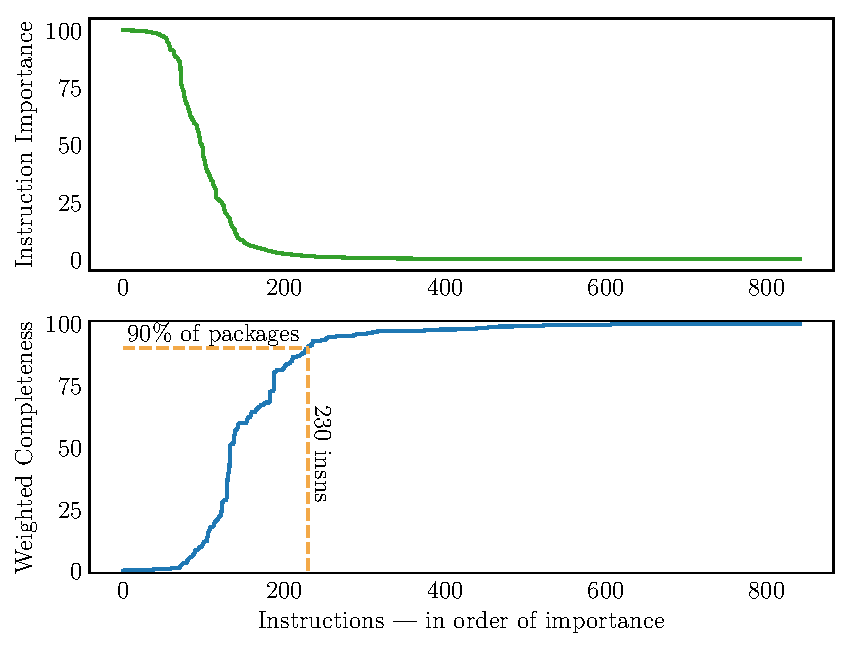
\includegraphics[width=0.5\linewidth]{figures/WCvMnem.pdf}
	\caption{ Instruction Importance (top): Distribution of instructions by percent of packages that need the instruction. Weighted completeness(bottom): What percent of packages can execute on a system that follows a greedy implementation strategy?}
	\label{fig:WCvMnem}
\end{figure}

Binary translation of a gargantuan ISA like Intel x86-64, which has
\textasciitilde{}3800 instructions, requires prioritizing development effort
on the most ``important'' instructions---trading completeness for simplicity
and a quicker development cycle.
For instance, the authors of VMware workstation describe an ``on-demand
implementation'' process, where the x86 binary translator focused on just the
instructions needed for a target OS; the entire ISA was never supported, and
guest OSes such as OS/2 did not work~\cite{bugnion-workstation}.
Similarly, Amit et al.~\cite{amit-161} showed that KVM cannot correctly
implement certain obscure x86 behaviors in a guest OS.
Prioritizing instruction support is a natural and ubiquitous engineering
trade-off. Some instructions appear in program binaries more frequently than
others, e.g., the \texttt{MOV} instruction (used to move data) is the most
common \texttt{x86-64} instruction. On the contrary, the \texttt{VFM\-ADD\-SD}
instruction, used to express a fused multiplication and addition operation, is
relatively rare. Further, many instructions perform similar operations, albeit
with subtle distinctions.

What, then, is the basis for assigning priority to instructions? Common
approaches include analyzing benchmark suites~\cite{SPEC2017-ab,Henning2006-ns,
bienia11benchmarking}, or execution traces collected in target
environments~\cite{elastictraces-axa}.
The ad-hoc nature of this approach leaves many useful questions unanswered:
Is the chosen test suite actually representative?
What is the path of least effort to support a new ISA in a software tool?
What minimum set of instructions must be implemented to run at least one
application? What instruction sub-set is sufficient to run the majority of
deployed applications?

To paraphrase Hennessy and Patterson~\cite{Patterson-textbook}, the best thing
to measure is what actually runs on the user's system.
This chapter will present and analyze a dataset collected from static analysis
of all x86-64 ELF binaries in the Ubuntu 16.04 GNU/Linux distribution.
We leverage package installation frequency, an approximation of a package's
importance to users, from Ubuntu and Debian popularity contest
data~\cite{ubuntu-popcon-tj,debian-popcorn-sb}, to infer the relative
importance of an instruction from the percentage of binaries on a given
system that contain that instruction.
We adapt metrics from a prior study of OS API compatibility~\cite{Tsai2016-zq},
specifically, \textit{instruction importance} --- the relative importance of
a given instruction, and \textit{weighted completeness} --- the completeness
of a system that implements a subset of the ISA.

Figure~\ref{fig:WCvMnem} is illustrative of the kinds of analysis our dataset
is useful for. The data presented in the figure shows that a small number of
instructions, about 30, are indispensable to all applications. The top 100
most important instructions are used by \texttildelow{}88\% of all packages.
Importance drops to 10\% by the 200~\textsuperscript{th} instruction, and 1\%
by the 240~\textsuperscript{th} instruction.

\noindent This chapter will present:
\begin{itemize}[noitemsep, topsep=0pt, leftmargin=1em, labelwidth=*, align=left]
\item An instruction occurrence dataset gathered using static analysis of
	9,337 open-source applications in the Ubuntu 16.04 repositories.
\item Evaluation of conventional wisdom about ISA usage.
\item An iterative plan for developing new tools that use the
	\texttt{x86-64} ISA.
\item Empirical validation of standard benchmarks.
\item An instruction occurrence data visualization tool, and the analysis framework used in this study are available at
	\url{http://x86instructionpop.com/}.
\end{itemize}

This chapter will be drawn from joint work~\cite{x86-systor} with Bhushan
Jain, Chia-che Tsai, Michael Ferdman and Donald E. Porter.
% !TeX root = dissertation.tex
\chapter{ISA virtualization is untenable for GPUs}
\label{sec:trillium}

\def\gpuvmdef{\textsc{GPU\-vm-default}\xspace}
\def\gpuvmopt{\textsc{GPU\-vm-opt}\xspace}
\def\trxc{\textsc{Xen-SVGA}\xspace}
\def\trxc{\textsc{Xen-SVGA}\xspace}
\def\trillium{\textsc{{T}rillium}\xspace}
\def\Trillium{\textsc{{T}rillium}\xspace}
\def\trxd{\Trillium}
\def\apigpu{\textsc{API-remote-GPU}\xspace}
\def\apicpu{\textsc{API-remote-CPU}\xspace}
\def\shadowpipe{\texttt{shadow-pipe}\xspace}
\def\Shadowpipe{\texttt{Shadow-pipe}\xspace}
\def\vframework{\textsc{{IEMTS}}\xspace}

% !TeX root = ../dissertation.tex

In many parallel computing domains, compute density and
programmability~\cite{nvidia_cuda, stone2010opencl, gregory2014c++} have
made GPUs the clear choice for efficiency and performance~\cite{gpu_apps}.
Popular machine learning frameworks such as Caffe~\cite{jia2014caffe},
Tensorflow~\cite{abadi2016tensorflow}, Microsoft CNTK~\cite{yu2014cntk},
and Torch7~\cite{collobert2011torch7} rely on GPU acceleration heavily.
GPUs have made significant inroads in HPC as well: five of the top seven
supercomputers in the world are powered by GPUs~\cite{top500-Nov2018}.

Despite much prior research~\cite{rossbach16vee, kaveri16vee,
cc-numa-gpu-hpca15, abhishek-ispass16} on GPGPU virtualization, practical
options currently available to providers of virtual infrastructure all involve
bypassing the hypervisor. The most commonly adopted technique is to dedicate
GPUs to single VM instances via PCIe pass-through~\cite{AWS-gpu,gVirt},
thereby giving up the consolidation and fault tolerance benefits of
virtualization. More recently, industry players such as VMware, Dell and
BitFusion have introduced user-space API-remoting~\cite{bitfusion-whitepaper,
kim2012snucl, rCUDAnew, vmCUDA,rCUDA} based solutions as an alternative to
pass-through. API-remoting recovers the consolidation and encapsulation
benefits of virtualization but bypasses hypervisor interposition. The absence
of hypervisor interposition results in multiple disjoint resource managers
(the remote user-space API executor and the hypervisor) with no insight into
each others' decisions, thereby leading to poor decision making, and
priority-inversion problems~\cite{rossbach2011ptask}.

To recover hypervisor interposition while maintaining low-overhead, we explore
retrofitting GPGPU support into a virtual GPU device: We added support for
OpenCL to an implementation of the SVGA~\cite{dowty2009gpu} design in Xen, by
implementing the key missing component---a compiler for SVGA's TGSI virtual
ISA.
This effort helped us realize that because GPUs already support vendor-specific
virtual ISAs (vISAs), the additional vISA provides little benefit.
In fact, we found that it harms performance by necessitating a translation
layer that obscures the program's semantic information from the final
vendor-provided compiler.
Drawing on this lesson, we adapted \Trillium to take a more flexible approach
to ISA virtualization: eliding it entirely when the host GPU stack bundles a
compiler (most do), and using LLVM IR, when necessary, to provide a common
target for GPGPU drivers.

\Trillium represents an unexplored point in the GPGPU virtualization design space:
hypervisor-mediated API-remoting.
\Trillium is an existence proof of a viable alternative design that preserves desirable
virtualization properties such as consolidation, hypervisor interposition, isolation,
encapsulation, etc., without requiring full hardware virtualization.
% \Trillium interposes one of the lowest layers in the guest GPGPU stack: the Gallium3D pipe-driver.
% Typically, this results in a single OpenCL call being broken into multiple pipe-driver
% calls.
\Trillium outperforms a full virtualization system from the literature
by up to 14$\times$ (5.5$\times$ on average) and outperforms the para-virtual
SVGA-like design by as much as 7.3$\times$ (5.4$\times$ on average).
% \hyu{Should mention the slowdown compared with pure user-space API remoting?}

% This enables efficient interposition through a low-overhead communication channel to the hypervisor --- shared memory.
% Since the SVGA design uses a virtual ISA (vISA),

% It also requires that compilers that implement these
%translations be competitive with GPU vendor compilers.  The missing
%ISA must be replaced by something: we consider variants that treat the
%front end code as IR, refactoring compilation to the hypervisor, and a
%variant that uses LLVM IR as the virtual ISA.  The emerging Vulkan
%framework~\cite{Vulkanspec} suggests an ISA called SPIR-V as a replacement; we do not
%evaluate a variant that uses SPIR-V.

%We consider variants of the design that address the now absent TGSI
%At a minimum,
%induced by the need to translate a guest GPU ISA
%to a single hypervisor-supported virtual ISA, and subsequently re-translate it
% to the ISA of the system's physical GPU.

% Flexible interposition and strong isolation mechanisms
% are critical for device management: a virtualization layer's
% primary goal is to enable isolated sharing across VMs. However, virtualization
% of the GPU ISA serves only compatibility, and often does so redundantly
% as GPGPU frameworks like OpenCL and CUDA subsume compilers
% into the device driver. Recognizing this redundancy,
% Trillium elides GPU ISA virtualization, relegating the translation from GPU
% source code to physical GPU ISA to the hypervisor-resident driver. While the separation of
% concerns requires a compiler in host or hypervisor, it vastly reduces
% complexity, eliminates a redundant translation layer, and ensures that the
% GPU compiler has a high-fidelity view of the target hardware, restoring
% optimization opportunities sacrificed by a design that relies on multiple translations.
%Moreover, raising the level of abstraction for the GPU ABI from an ISA to
%source code is not as heretical as one might think: OpenCL drivers are generally
%expected to ship with an integrated source-level compiler.

% We evaluated a \Trillium prototype against systems %from the literature
% representative of full virtualization, API remoting, and VMware's SVGA.


% \noindent This paper make the following contributions:
% \begin{compactitem}
% \item We show that API-remoting does not have to be done entirely in user-space
%   and that it can be hypervisor-mediated with minimal loss of performance.
%   % \hyu{With tolerable loss? Compared with native run, this statement is not true. At least the impl\&measurement in this paper don't prove this point.}
% \item We implement GPGPU support for an SVGA-like design in the Xen
%   hypervisor, by completing a long-missing element---the TGSI compiler---%
%   in order to leverage OpenCL support provided by the Mesa/Gallium graphics
%   stack for Linux, via the Clover~\cite{GalliumCompute-web} project.
% \item We propose an improved design called \Trillium that
%   removes the necessity for the vISA defined by SVGA resulting in dramatic
%   performance improvements.
% \item We provide the first (to our knowledge) comprehensive empirical and
%   qualitative comparison of a wide range of fundamental virtualization
%   techniques from the literature.
% \end{compactitem}

% !TeX root = ../dissertation.tex

\section{Background}
\label{sec_background}

Existing GPU virtualization solutions~\cite{dowty2009gpu, VGML} support
graphics frameworks like Direct3D~\cite{directX}, OpenGL~\cite{openGLspec}.
In principle, there should be no fundamental difference between GPU virtualization for graphics versus \emph{compute} workloads.
% because ``compute shaders'' are implemented by the hardware as an additional
% stage in the graphics pipeline~\cite{gpu_shader}.
In practice, they have significantly different goals:
For graphics, virtualization designs target an interactive frame rate (18-30
fps~\cite{frame_rate}). For GPGPU compute, virtualization designs must
preserve the raw speedup achieved by the hand-optimized GPGPU application,
which is a considerably harder target to hit. As a result, GPGPU virtualization
remains an open problem. While graphics devices have long enjoyed well-defined
OS abstractions and interfaces~\cite{winGDI},
% the same is not true for GPGPU \emph{compute} devices:
research attention to OS abstractions for GPGPUs~\cite{rossbach2011ptask, dandelion, silberstein2013gpufs, timegraph, gdev, gpunet} has yielded little consensus.
% Furthermore, persistent vendor-specificity of programming frameworks continue to frustrate both interposition and compatibility.

\begin{figure}[!th]
	\centering
	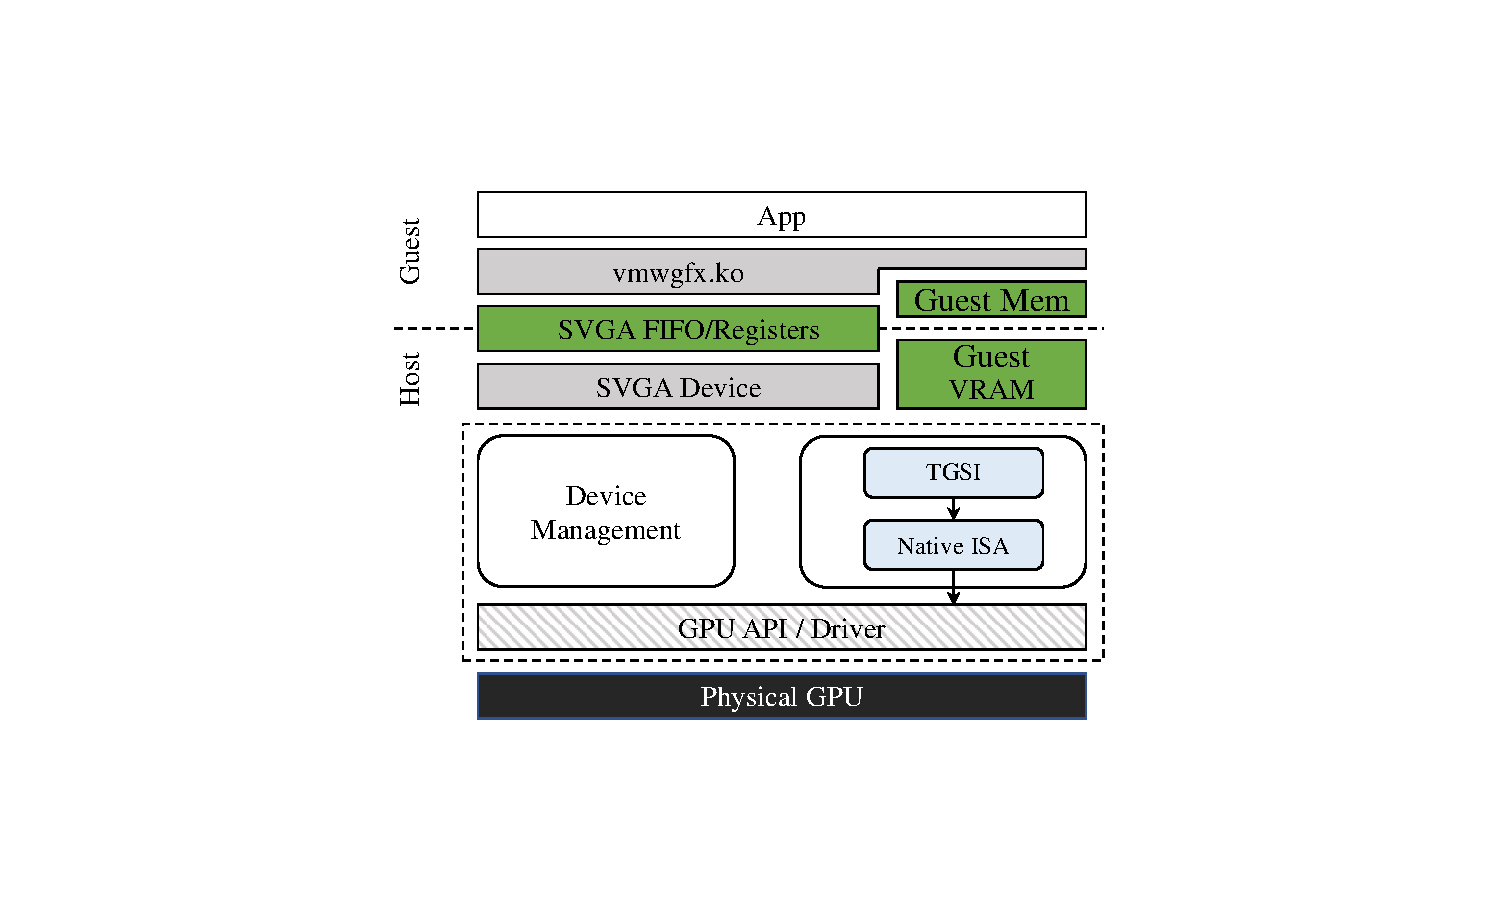
\includegraphics[width=.75\linewidth,trim={6cm 3cm 6cm 3cm},clip]{trillium/images/svga.pdf}
	\caption{{\footnotesize The design of SVGA.}}
	\label{fig_svga} \end{figure}

\subsection{SVGA}
\label{sec:svga}

SVGA~\cite{dowty2009gpu} remotes DirectX and OpenGL over an emulated (software) PCIe device.
The SVGA virtual device behaves like a physical GPU, by exporting virtual resources
in the form of registers, extents of guest memory accessible to the virtual device,
and a command queue.
I/O registers (used for mode switching, IRQs, memory allocation) are mapped
in an interposed PCIe Base Address Register (BAR) to enable synchronous emulation.
Access to GPU memory is supported through asynchronous DMA.
Figure~\ref{fig_svga} presents an overview of SVGA.

SVGA combines many aspects of full-, para-virtual and API remoting designs.
Unmodified guests can transparently use SVGA as a VGA device, making full
virtualization possible where necessary. However, access to GPU acceleration
requires para-virtualization through VMware's guest driver.
% Like a physical GPU,
SVGA processes commands from a memory mapped command queue;
% unlike a physical GPU, the command queue can be
% directly accessed by the hypervisor,
the command queue functions as a transport layer for protocols
between the guest graphics stack and the hypervisor.

SVGA uses the DirectX~\cite{directX} API as its internal protocol, thereby
realizing an API-remoting design. The transport layer and protocol are
completely under the control of the hypervisor, enabling many of the benefits
of API-remoting while ameliorating its downsides. However, using the DirectX
API as a transport protocol requires that
the driver and hypervisor translate guest interactions into DirectX
whether they are natively expressed in DirectX or not.
Coupling the transport layer with a particular version of the DirectX protocol has led to
serious complexity and compatibility \textit{challenges}: supporting each new version of the API
takes many person-years (VMware introduced support for DirectX 10 (introduced in 2006)
in 2015!).
SVGA also supports a virtual GPU ISA called TGSI~\cite{tgsi}.
% Originally developed for graphics,
TGSI maps naturally to the graphics features of the ISAs it was
originally designed to encapsulate, but has failed to keep up with
GPU ISAs that have evolved to support general purpose computation primitives.
% , TGSI has failed to evolve with it.

%SVGA's design for marshaling guest graphics stack
%calls to and from the DirectX API is essential to providing
%interactive graphics performance.
%However, the choice of a single API forces translation
%to and from other framework APIs,
%and mapping TGSI to all possible physical GPU ISAs
%creates a significant compatibility problem which over time
%has introduced staggering software complexity;
%SVGA has consequently failed to keep up with evolution of
%graphics frameworks despite monumental engineering effort.

\subsection{Mesa3D OpenCL Support}

The Mesa3D Graphics Library~\cite{mesa} is an open-source graphics
framework that implements graphics runtime libraries (e.g., OpenGL~\cite{openGLspec}, Vulkan~\cite{Vulkanspec}, Direct3D~\cite{directX}, and OpenCL~\cite{stone2010opencl})
% It is the default graphics stack
on most GNU/Linux installations.
% Mesa3D includes support for  and others.
It also includes official device drivers, written in a common framework, Gallium3D~\cite{gallium}, for Intel and AMD GPUs.
Support for NVIDIA GPUs is provided via reverse-engineered open-source Nouveau driver. Gallium3D imposes TGSI as the common
virtual ISA for compute shaders, and decomposes drivers into two
components: \textit{state trackers}, which keep track of the device
state, and \textit{pipe drivers}, which provide an interface for
controlling the GPU's graphics pipeline.
% (e.g. translate the state, shaders, and primitives into something that the hardware understands).
% Effort is underway to replace TGSI with
% SPIR-V and LLVM IR, but it wasn't mature when we undertook this project.

OpenCL support was first introduced in Mesa3D 9.0 with the release of the
Clover state tracker.
% Clover supports OpenCL~1.1 and was mainly contributed by AMD developers.
It was envisioned that Clover would leverage the LLVM~\cite{lattner2004llvm}
compiler to lower the OpenCL source to TGSI. Despite much effort by the
open-source community~\cite{old_llvm_tgsi1,old_llvm_tgsi2}, an LLVM TGSI back-end
has remained incomplete.
% Contributed by AMD developers and open-source community, Clover supports OpenCL~1.1 on most AMD GPUs.
% However, because AMD started to focus upon their ROCm compute platform~\cite{amd_rocm},
% Clover has not kept up with the fast upgrades of vendor hardware and
% software systems.
Clover currently supports an incomplete set of OpenCL~1.1 APIs on AMD GPUs and fails to operate
correctly on NVIDIA GPUs.

\subsection{GPU ISAs and IRs}

GPU front-end compilers produce code in virtual ISAs (NVIDIA PTX and LLVM IR for AMD) which are subsequently finalized using JIT compilers in the GPU driver to the native ISA (SASS and GCN).
The vISA remains stable across generations to preserve compatibility, while
the physical ISA is free to evolve. TGSI, the virtual ISA used in both the Mesa
stack and SVGA, plays a similar role---enabling interoperability
between graphics frameworks and GPUs from different vendors.
An improved virtual ISA, SPIR-V, has been proposed as a new standard~\cite{Vulkanspec} and an effort is under way to replace TGSI with SPIR-V in the Mesa3D stack.
%When standardization works, interoperability and compatibility are much easier
%to achieve.
%IRs, such as TGSI, designed by driver frameworks end up being too intertwined
%with their frameworks to keep up with the fast pace of evolution in the
%HW, or don't achieve critical mass.

LLVM has become the de-facto standard for building compilers:
both NVIDIA and AMD use it to implement their virtual ISA compilers,
as do all the compilers in the Mesa stack including the TGSI compiler we implemented.
LLVM IR is in a unique position to become a standard IR.
%The framework supports a wide array of front-end languages including CUDA and OpenCL among others, and a wide array of back-ends as well, including other IRs like SPIR-V.

%% Intermediate Representations are incredibly useful tools to hardware vendors, enabling them to simultaneously:
%% \begin{compactitem}
%% \item preserve backward compatibility without compromising innovation at the ISA. By having a publicly available ISA, that has longevity, and can be then be translated to a set of instructions that doesn't need to be preserved across generations
%% \item have the ability to reoptimize legacy code for new HW without having a dependency on the high level toolkit that generated the code in the first place
%% \item have the freedom to optimize their hardware any way they see fit without having to worry about the effect of said optimizations on the ISA
%% \item simplify their tool-chain building process by having to only modify
%% one piece (the finalizer: the piece that translates from IR to physical ISA) with each new generation of HW
%% \item leverage open source frameworks like LLVM without having to give up their secret sauce
%% \end{compactitem}
%% Given these properties, it comes as no surprise that both AMD and Nvidia have
%% both a public virtual ISA that is stable across generations i.e. IL and PTX
%% respectively, and a physical ISA that is free to evolve with each generation
%% of hardware, i.e. GCN and SASS respectively. IRs are of great interest to
%% in the realm of virtualization because an IR that is expressive enough to be
%% able to take advantage of new HW developments, while also being universally
%% accepted by all the competing parties will make a wonderful GPGPU virtualization primitive.

%% As is often the case in a space where competition is fierce, standardization
%% is hard to come by. Despite efforts by standards organizations~\cite{Vulkanspec} to convince competing parties to find a middle ground, so as to give tool
%% writers some semblance of sanity, no clear standard IR has emerged in the
%% GPGPU realm. SPIR-V~\footnote{https://www.khronos.org/spir/} is the latest
%% challenger to walk this gauntlet.

%% IRs, such as TGSI, designed by driver frameworks end up being too intertwined
%% with their frameworks to keep up with the fast pace of evolution in the
%% HW, or don't achieve critical mass.

%% Interestingly, an unlikely candidate may have emerged that is viable as a
%% virtualization primitive: LLVM IR. As a function of being the compiler
%% framework that both Nvidia and AMD use to implement their virtual ISA
%% compilers, LLVM IR is in a unique position to be the candidate IR for GPGPU
%% virtualization frameworks. The framework supports a wide array of front-end languages including CUDA and OpenCL among others, and a wide array of back-ends as well, including other IRs like SPIR-V.

% \input{framework-dims}


% !TeX root = ../dissertation.tex
\section{Design}
\label{sec_design}
\label{sec:trillium_design}

\Trillium exports an abstract virtual device and a para-virtual guest driver,
which we use to interpose and forward the OpenCL and CUDA APIs to the host.
Unlike SVGA, which requires translation
layers to ensure that all graphics frameworks APIs can be mapped to the SVGA protocol,
Trillium forwards the lowest layer in the GNU/Linux Graphics stack: the pipe-driver,
effectively remoting OpenCL/CUDA API calls in the guest to the OpenCL/CUDA library in the host.

%\Trillium is composed of a virtual GPU device, and a para-virtual guest driver
%which we use to interpose and forward a GPGPU API through the virtual
%device implementation to the host. Unlike SVGA, which requires translation
%layers to map graphics APIs to the SVGA protocol, Trillium forwards
%Mesa3D pipe-driver functions directly, effectively remoting an OpenCL API
%implementation in the Mesa stack to an OpenCL implementation in the host.

%% \item The historical approach of translating/tunneling other graphics APIs
%% 	over the SVGA protocol is unnecessary, and the protocol can simply be
%% 	extended directly with GPGPU APIs without compromising
%% 	other important properties of the design.

% \Trillium is heavily influenced by the SVGA design, but
Our experience implementing the required TGSI vISA support in the Mesa
graphics stack led us to believe that the TGSI layer is unnecessary.
Not only does this translation introduce additional complexity in the guest
stack, it also hurts performance, as we demonstrate in Section~\ref{sec:eval}.
The guest OpenCL compiler cannot target the native GPU architecture,
and semantic information is lost to the host compiler.
% Because SVGA's native ISA is TGSI, supporting GPGPU workloads in SVGA requires
% GPU code to be expressed in TGSI, rather than in the ISAs produced
% by vendor-specific runtimes (e.g. CUDA's \texttt{PTX} and
% \texttt{SASS}, or AMD's \texttt{SPIR}).
Further, while incorporating a TGSI compiler is possible in open frameworks like OpenCL,
the task is significantly more daunting for closed frameworks like CUDA.
Attempts to translate between TGSI and NVIDIA SASS in the reverse-engineered Nouveau driver
understandably results in code that is significantly less performant
than that produced by the proprietary stack.

\Trillium takes a different approach:
% rather than build a compiler for guest to a virtual ISA which must then be translated in the hypervisor,
% of the production compiler for the actual physical device and
\Trillium forwards API calls for compiling OpenCL code to the hypervisor.
The OpenCL compiler in the host OpenCL framework
(optimized for the physical hardware by the hardware vendor)
is invoked on the forwarded OpenCL code to lower it directly to the physical device ISA.
% If the host OpenCL driver does not support a compiler, \Trillium uses LLVM IR as the virtual ISA.

%\begin{figure}[!th]
%	\centering
%	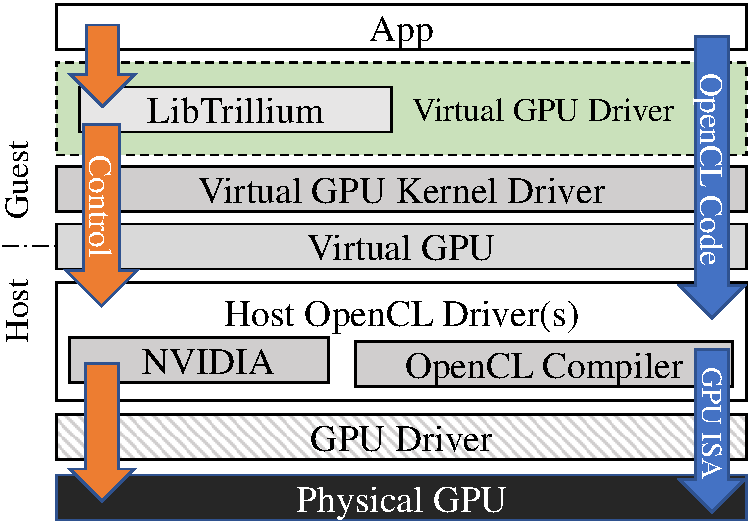
\includegraphics[width=.8\linewidth,trim={0 0 0 0},clip]{images/design/trillium_design.pdf}
%	\caption{{\footnotesize The design of \Trillium.
%            \cjr{FIXME: get designs in position as discussed with Hangchen. }}}
%	\label{fig_trillium} \end{figure}

Figure~\ref{fig_trillium} shows the Trillium design layers in a
generic hypervisor stack. The OpenCL API is forwarded from the
driver similar to the SVGA model.  The OpenCL compute kernel (to be
run on the GPU), can be passed through to the host via hypercalls in
the driver, without being translated to any vISA, where it will
be translated and optimized for the physical GPU in a virtual appliance (Dom~2 in Figure~\ref{fig_trillium}).

\Trillium does not currently guarantee performance isolation and relies on the hardware scheduler.
% task is handed to the hardware.
Performance isolation can easily be implemented via a rate-limiting API scheduler in the
hypervisor, such as in GPUvm~\cite{GPUvm}.

%% \aak{Chris, what level of detail do you want to go to? I'm keeping it minimal
%% here so as to not risk de-anonymizing you. Mentioning that you built this model
%% at VMware will bring questions of why we didn't measure that system instead.}

% \begin{figure}[!th]
% 	\centering
% 	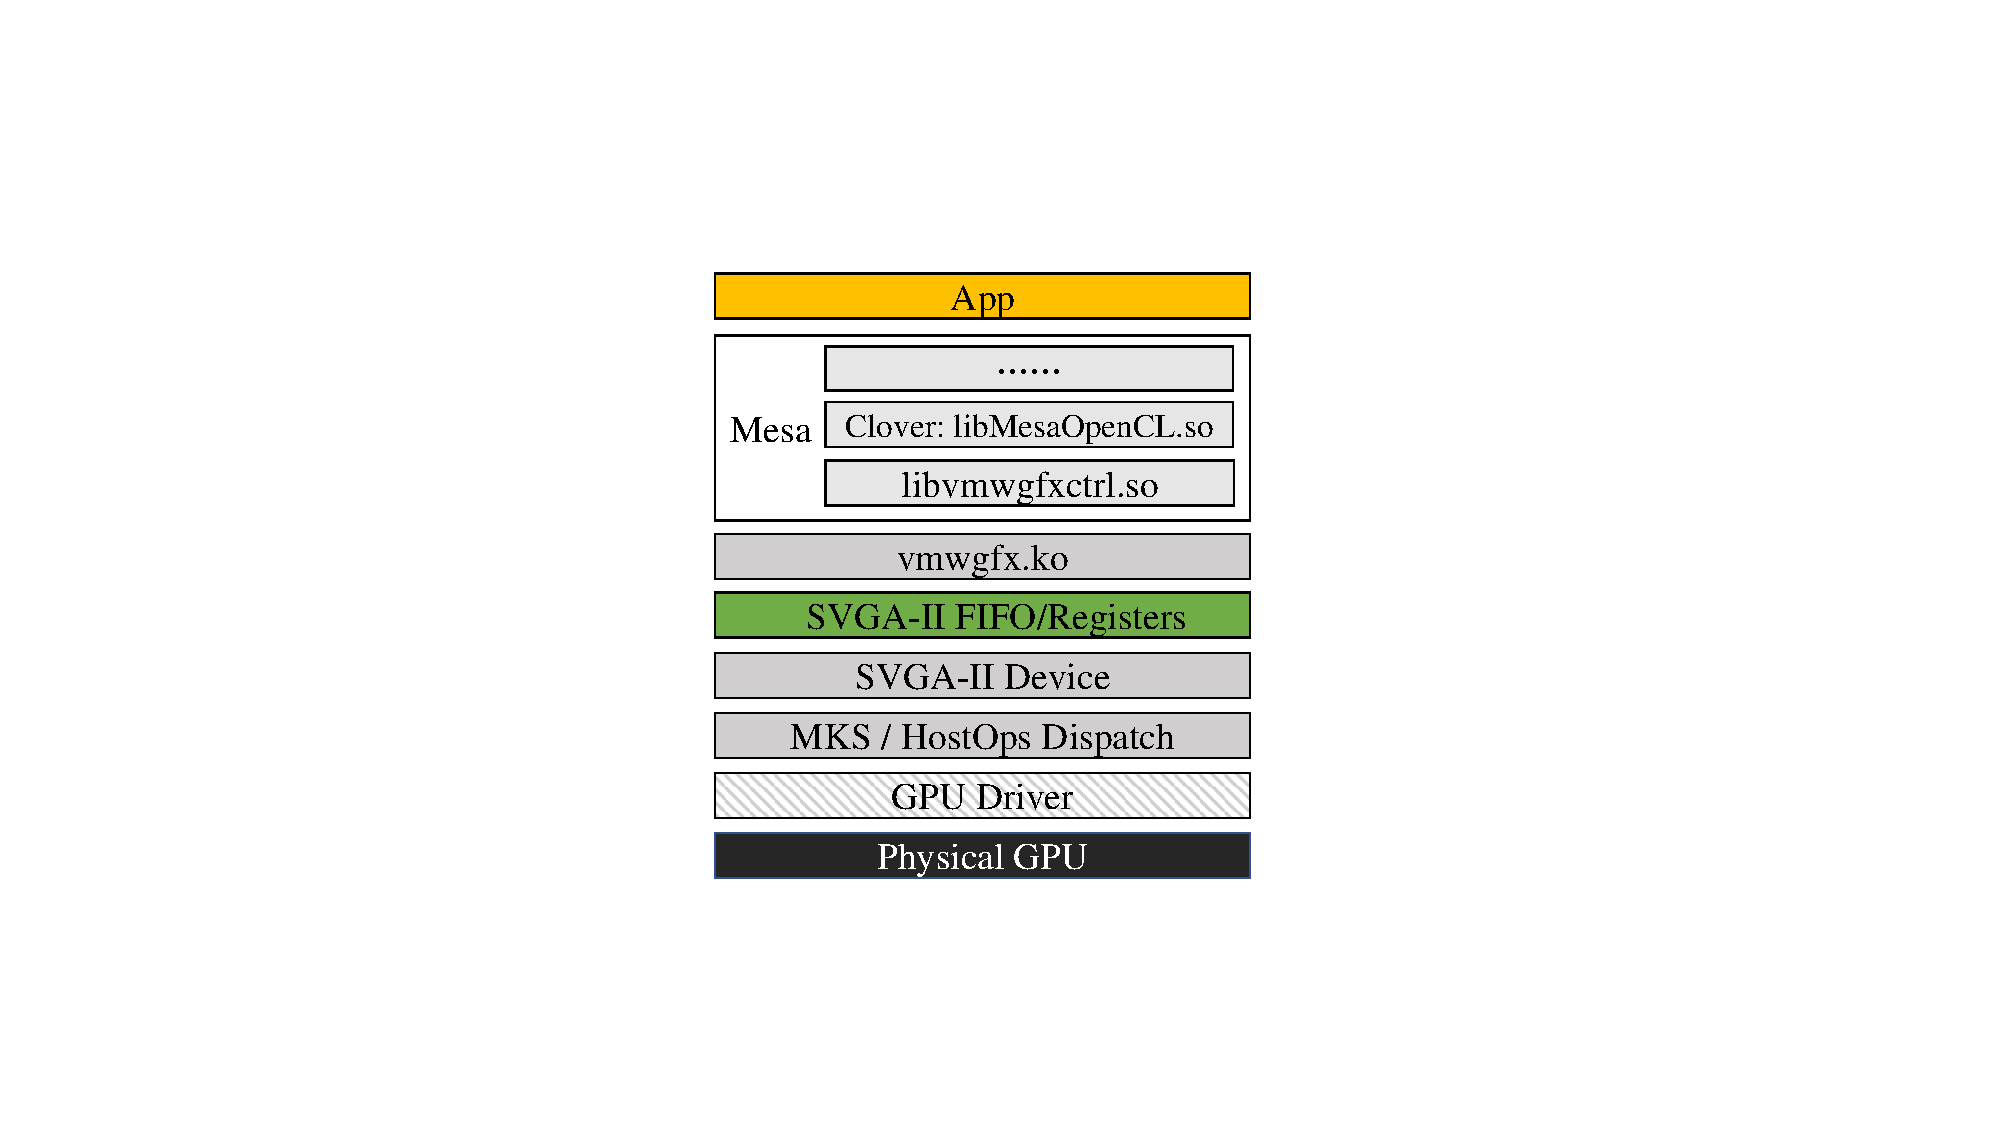
\includegraphics[width=\linewidth,trim={9cm 4cm 9cm 4.5cm},clip]{images/trillium/trillium_classic_single_node.pdf}
% 	\caption{{\footnotesize The design of Trillium Classic.}}
% 	\label{fig_trillium_classic2} \end{figure}


% \subsection{Impact of GPU virtual ISAs}


% % \begin{table}[!th]
% % 	\centering
% % 	\begin{tabular}{l|l|l|l|l|}
% % 		\cline{2-5}
% % 		& Init & MemCpy & Kernel & Total \\ \hline
% % 		\multicolumn{1}{|l|}{ocl+mesa} & \multicolumn{1}{r|}{5.4x} & \multicolumn{1}{r|}{6x} & \multicolumn{1}{r|}{14.5x} & \multicolumn{1}{r|}{7x} \\ \hline
% % 	\end{tabular}
% % 	\caption{Slowdown of Clover OpenCL runtime.}
% % 	\label{tb_clover_slowdown}
% % \end{table}

% The design trades off compatibility: the goal of the virtual TGSI ISA
% for the virtual GPU is to function as universal IR, so that a guest
% compiler is able to produce code that can always be finalized below
% the virtualization layer to a native ISA for the physical GPU. While
% conceptually attractive, the design decision is only effective if
% components elsewhere in the stack (GPU runtimes, compilers, drivers,
% etc.) actually standardize on it.  At present, NVIDIA and AMD GPGPU
% stacks both suppport virtual and native ISAs, but \emph{different}
% ones, neither of which is TGSI, making TGSI effectively an additional
% layer of virtualization on the ISA. We also observe that because both
% AMD and NVIDIA compilers are built on LLVM, there is an opportunity
% for standardizing on LLVM IR as the common IR, which would naturally
% recover the compatibility ceded by the \Trillium design.

% !TeX root = ../dissertation.tex

\section{Implementing representatives of each virtualization scheme}
\label{representative}

Existing GPU virtualization solutions~\cite{dowty2009gpu, VGML} support
graphics frameworks like Direct3D~\cite{directX}, OpenGL~\cite{openGLspec}.
In principle, there should be no fundamental difference between GPU
virtualization for graphics versus \emph{compute} workloads: ``compute
shaders'' are implemented by the hardware as an additional stage in the
graphics pipeline~\cite{gpu_shader}. In practice, they have significantly
different goals: For graphics, virtualization designs target an interactive
frame rate (18-30 fps~\cite{frame_rate}). For GPGPU compute, virtualization
designs must preserve the raw speedup achieved by the hand-optimized GPGPU
application, which is a considerably harder target to hit. As a result, GPGPU
virtualization remains an open problem. While graphics devices have long
enjoyed well-defined OS abstractions and interfaces~\cite{winGDI}, research
attention to OS abstractions for GPGPUs~\cite{rossbach2011ptask, dandelion,
silberstein2013gpufs, timegraph, gdev, gpunet} has yielded little consensus.
This section describes each of the systems that we chose to represent each of
the canonical virtualization schemes in our empirical analysis, and how we modified or implemented them.

\subsection{GPUvm}
As a representative of full and para-virtual schemes, we chose to study
GPUvm~\cite{suzuki2014gpuvm}, a Xen-based virtualization scheme for NVIDIA's
Kepler and Fermi GPUs. A simplified block-diagram representation is shown in
Figure~\ref{fig_gpuvm_basic}). GPUvm presents each VM with a GPU device model,
which is emulated in the privileged domain (Dom 0). Attempts to access the GPU
from all VMs are interposed via traps and are routed through a GPU Aggregator.
The  aggregator maintains shadow page tables, shadow channels, implements a
``fair share scheduler'', and modifies requests to enforce isolation. GPUvm
interposes on communication between guest device driver and the GPU device
model, by trapping and forwarding MMIO writes. The authors also explore a
number of optimizations: lazy shadowing, bar remap, para-virtualization, and
multi-call batching. GPUvm has not been maintained: The last release, in 2012,
is based on Xen 4.2.0 and runs on Fedora~16~\cite{yu2017fullvirt}. In order to
compare all of the representatives on the same modern platform, we ported
GPUvm to Ubuntu~16.04 with Xen~4.8.2.

\begin{figure}[!th]
	\centering
	\begin{subfigure}{.45\columnwidth}
		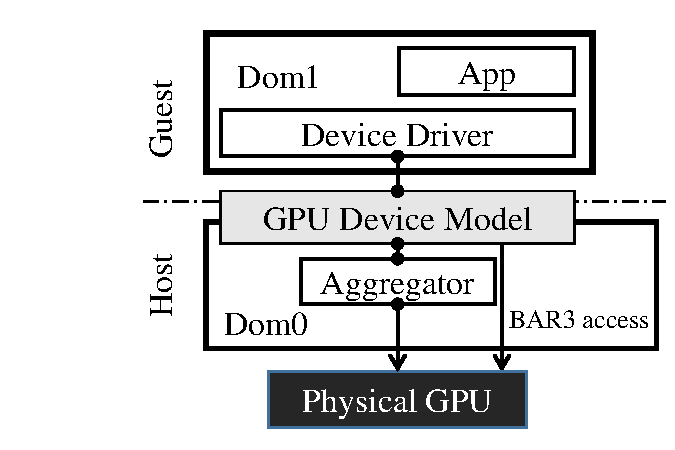
\includegraphics[width=\columnwidth,trim={2cm 0cm 0cm 0cm},clip]{trillium/images/design/gpuvm.pdf}
		\caption{{}}
		\label{fig_gpuvm_basic}
	\end{subfigure}\hfill
	\begin{subfigure}{.55\columnwidth}
		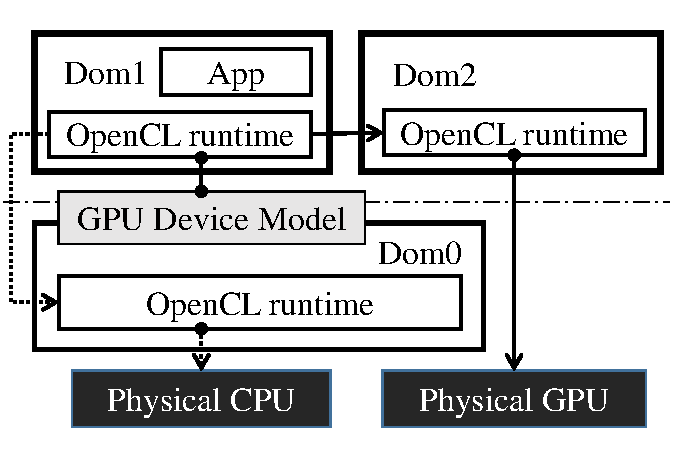
\includegraphics[width=\columnwidth,trim={0 0 0 0},clip]{trillium/images/design/api-remote.pdf}
		\caption{{}}
		\label{fig:api_remote}
	\end{subfigure}
	\caption{{\footnotesize Xen-based virtualizaton designs. (a) GPUvm. (b) User-space API remoting over RPC---dashed arrows indicate \apicpu, while solid ones indicate \apigpu.}}
\end{figure}

\subsection{User-space API remoting}

In order to faithfully mimic user-space API-remoting systems~\cite{rCUDA,
kim2012snucl,bitfusion-whitepaper}, we implemented a system on Xen that trapped
OpenCL API calls using a user-space shim library. These trapped calls were
then forwarded, via RPC, from one appliance VM (the ``client'') to another
appliance VM (the ``server''). Figure~\ref{fig:api_remote} shows the setup of
the two API-remoting schemes we considered: \apigpu and \apicpu.
The black arrows indicate the workflow of \apigpu, where the OpenCL server
ran the OpenCL commands on a physical GPU using the NVIDIA OpenCL framework.
The grey arrows show the \apicpu setup, where the OpenCL commands were
executed on a multi-core CPU (Intel CPU Xeon E5-2643) using the Intel OpenCL
SRB~5.0 framework. The remoting itself was accomplished using gRPC~1.6
(ProtocolBuffers~3.4.0) and inter-service communications were implemented over
XML-RPC~1.39. Lower-overhead data-movement techniques, such as zero-copy, can
be applied when both the client and the server are on a local machine, but
were not considered in our implementations.


\begin{figure*}[!th]
	\centering
	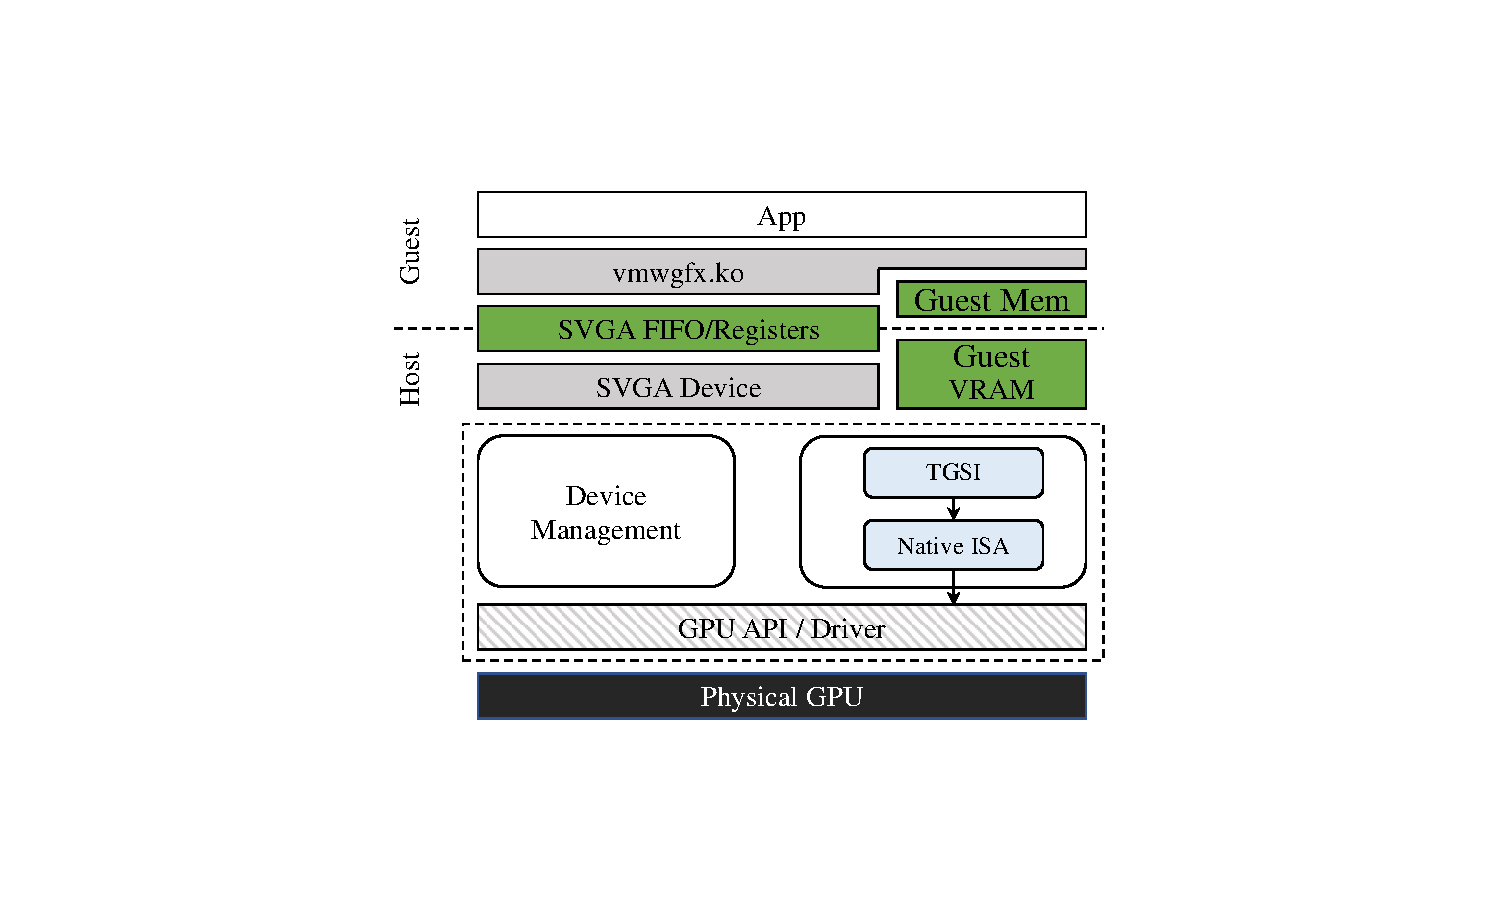
\includegraphics[width=.5\linewidth,trim={6cm 3cm 6cm 3cm},clip]{trillium/images/svga.pdf}
	\caption{{\footnotesize Stack diagram of the SVGA virtualization scheme.}}
	\label{fig_svga}
\end{figure*}

\subsection{SVGA}

SVGA~\cite{dowty2009gpu} remotes DirectX and OpenGL over an emulated (
software) PCIe device. The SVGA virtual device behaves like a physical GPU, by
exporting virtual resources in the form of registers, extents of guest memory
accessible to the virtual device, and a command queue. I/O registers (used for
mode switching, IRQs, memory allocation) are mapped in an interposed PCIe Base
Address Register (BAR) to enable synchronous emulation. Access to GPU memory
is supported through asynchronous DMA. Figure~\ref{fig_svga} presents an
overview of SVGA.

SVGA combines many aspects of full-, para-virtual and API remoting designs.
Unmodified guests can transparently use SVGA as a VGA device, making full
virtualization possible where necessary. However, access to GPU acceleration
requires para-virtualization through VMware's guest driver. As in a physical
GPU, SVGA processes commands from a memory mapped command queue; unlike in a
physical GPU, the command queue functions as a transport layer for APIs
between the guest graphics stack and the hypervisor.

SVGA uses the DirectX~\cite{directX} API as its internal protocol, thereby
realizing an API-remoting design. The transport layer and protocol are
completely under the control of the hypervisor, enabling many of the benefits
of API-remoting while ameliorating its downsides. However, using the DirectX
API as a transport protocol requires that the driver and hypervisor translate
guest interactions into DirectX whether they are natively expressed in DirectX
or not. Coupling the transport layer with a particular version of the DirectX
protocol has led to serious complexity and compatibility \textit{challenges}:
supporting each new version of the API takes many person-years (VMware
introduced support for DirectX 10 (released in 2006) in 2015!).

SVGA also relies on a virtual GPU ISA called TGSI~\cite{tgsi}. TGSI maps
naturally to the graphics features of the ISAs it was originally designed to
encapsulate, but has failed to keep up with GPU ISAs that have evolved to
support general purpose computation primitives. Further, mapping TGSI to all
possible physical GPU ISAs is a herculean task that was doomed from the outset.

\begin{figure*}[!th]
	\centering
	\begin{subfigure}{.5\linewidth}
		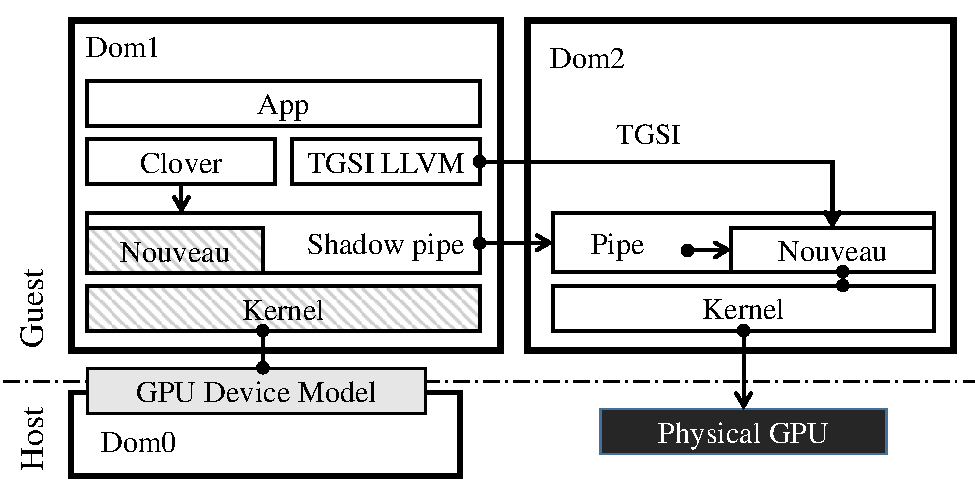
\includegraphics[width=\columnwidth,trim={0 0 0 0},clip]{trillium/images/design/xen-svga.pdf}
		\caption{{}}
		\label{fig_trillium_classic}
	\end{subfigure}\hfill
	\begin{subfigure}{.5\linewidth}
		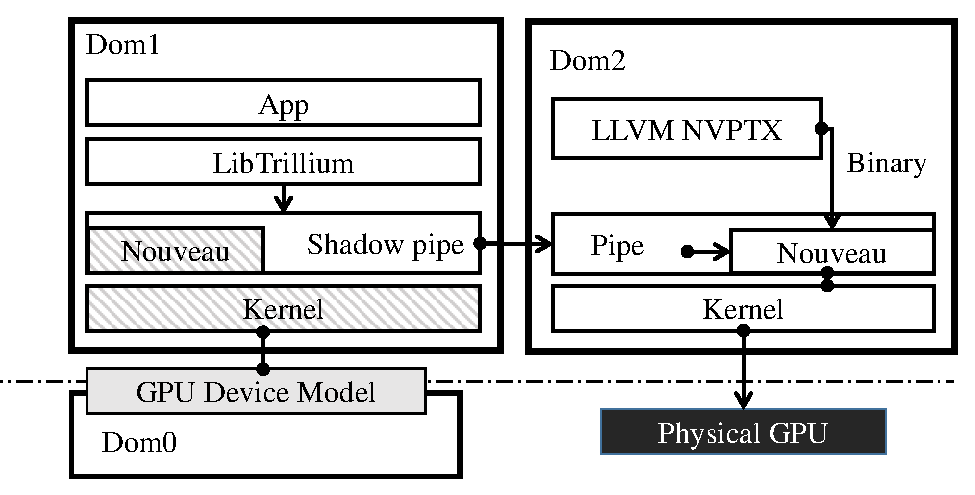
\includegraphics[width=\columnwidth,trim={0.6cm 0 0 0},clip]{trillium/images/design/trillium.pdf}
		\caption{{}}
		\label{fig_trillium_direct}
	\end{subfigure}
	\caption{{\footnotesize \XenSVGA and \Trillium designs. (a) \XenSVGA approximates the SVGA model extended to support GPU Compute. (c) The design of \Trillium with shadow pipe.}}
\end{figure*}

\subsection{\XenSVGA and \Trillium}

We initially implemented the SVGA~\cite{dowty2009gpu} model on Xen strictly
keeping with the original design: we implemented OpenCL support in a virtual
device and extended the Mesa stack with TGSI support (see Section~\ref{ssec:tgsi_backend} for details). The generated TGSI is sent to the host via
RPC, and then finalized to a binary that can be run on the physical NVIDIA GPU
using the open source Nouveau driver. This faithful implementation, hereafter
called \XenSVGA, is used in our study as a representative of the original SVGA
design. \XenSVGA is shown in Figure~\ref{fig_trillium_classic}.

In order to test our hypothesis about vISAs, we modified \XenSVGA to elide the
TGSI compiler, thus arriving at \Trillium. \Trillium forwards API calls for
compiling OpenCL code to the hypervisor. The OpenCL compiler in the host
OpenCL framework (optimized for the physical hardware by the hardware vendor)
is invoked on the forwarded OpenCL code to lower it directly to the physical
device ISA. Figure~\ref{fig_trillium_direct} shows the Trillium design in the
Xen hypervisor stack. The OpenCL API is forwarded from the driver similar to
\XenSVGA. The OpenCL compute kernel (to be run on the GPU) is passed through to
the host via hypercalls in the driver, without being translated to TGSI, where
it will be translated and optimized for the physical GPU in a virtual
appliance (Dom~2 in Figure~\ref{fig_trillium_direct}).

\XenSVGA and \Trillium export an abstract virtual device and a para-virtual
guest driver, which we use to interpose and forward the OpenCL and CUDA APIs
to the host. Unlike SVGA, which requires translation layers to ensure that all
graphics frameworks APIs can be mapped to the SVGA protocol, \XenSVGA and
\Trillium forward the lowest layer in the GNU/Linux Graphics stack: the
pipe-driver, effectively remoting OpenCL/CUDA API calls in the guest to the
OpenCL/CUDA library in the host.

\XenSVGA and \Trillium, implement API-forwarding in a custom pipe-driver in
Gallium3D, that we call \shadowpipe. We chose to forward the pipe-driver as it
is presents a narrow interposition interface in the graphics driver. However,
given that each OpenCL API call is decomposed into many different pipe-driver
calls, other APIs higher up in the graphics stack may be better suited for
interposition. The \shadowpipe is in the \textit{application domain}'s graphics
stack, and shims the pipe-driver interface as RPC calls to the actual Nouveau
pipe-driver in the \textit{privileged domain}.

\XenSVGA and \Trillium manage user-level contexts, command queues and memory
objects. While \XenSVGA relies on our TGSI compiler to translate the input
OpenCL GPGPU kernel to TGSI in the application domain, \Trillium skips the
compilation phase. Instead, the OpenCL kernel is forwarded to the privileged
domain via RPC, where it is parsed and compiled by the LLVM NVPTX back-end in
parallel. This binary is then loaded onto the GPU when the pipe-driver hits
the binary loading phase. \Trillium can also emit LLVM IR if an OpenCL
compiler is not available in the host.

Our implementation relies on gRPC as a transport mechanism between the guest
and the host, as an implementation convenience. As zero-copy transfer~\cite{
chu1996zero,tezuka1998pin} and hypercall~\cite{ram2010redesigning} mechanisms
are well-studied, and a production-ready version of \Trillium would rely on
these mechanisms, we measure and remove transport overhead from our reported
measurements in Section~\ref{sec:trilliumeval}.
The overheads stem from remoting calls to the privileged domain over the
network, which is especially significant since a single OpenCL API call may be
decomposed into many pipe-driver APIs, and from the large amount of kernel
input data that must be copied between VMs.
\XenSVGA and \Trillium do not currently guarantee performance isolation,
although this can easily be implemented via a rate-limiting API scheduler in
the hypervisor, as in GPUvm~\cite{GPUvm}.

\subsubsection{Mesa3D OpenCL Support}

The Mesa3D Graphics Library~\cite{mesa} is an open-source graphics framework
that implements graphics runtime libraries (e.g., OpenGL~\cite{openGLspec},
Vulkan~\cite{Vulkanspec}, Direct3D~\cite{directX}, and OpenCL~\cite{
stone2010opencl}) on most GNU/Linux installations. It also includes official
device drivers, written in a common framework, Gallium3D~\cite{gallium}, for
Intel and AMD GPUs. Support for NVIDIA GPUs is provided via reverse-engineered
open-source driver, Nouveau. Gallium3D imposes TGSI as the common virtual ISA
for compute shaders, and decomposes drivers into two components: \textit{state
trackers}, which keep track of the device state, and \textit{pipe drivers},
which provide an interface for controlling the GPU's graphics pipeline (e.g.
translate the state, shaders, and primitives into something that the hardware
understands). Effort is underway to replace TGSI with SPIR-V and LLVM IR, but
it wasn't mature when we undertook this project.

OpenCL support was first introduced in Mesa3D 9.0 with the release of the
Clover state tracker. Clover supports OpenCL~1.1 and was mainly contributed by
AMD developers. It was envisioned that Clover would leverage the LLVM~\cite{
lattner2004llvm} compiler to lower the OpenCL source to TGSI. Despite much
effort by the open-source community~\cite{old_llvm_tgsi1,old_llvm_tgsi2}, an
LLVM TGSI back-end has remained incomplete. Clover currently supports an
incomplete set of OpenCL~1.1 APIs on AMD GPUs and fails to operate correctly
on NVIDIA GPUs.

\subsubsection{LLVM TGSI Back-end}
\label{ssec:tgsi_backend}
While Clover provides the library for the OpenCL application to link against,
most of the compilation is handled by invoking the OpenCL and C++ front-ends
of the LLVM~\cite{lattner2004llvm} compiler framework. Clover provides much of
the front-end infrastructure required to support GPGPU computing in \XenSVGA
and \Trillium. However, LLVM lacks a working TGSI back-end, which presented a
challenge for \XenSVGA.

In order to support OpenCL in \XenSVGA, we implemented an LLVM TGSI back-end.
While the TGSI back-end is not yet mature, we added support for a majority of
the 32-bit integer and floating point operations, intrinsics, memory barriers,
and control flow. Using this backend we were able to compile and run 10 out of
the 12 Rodinia benchmarks~\cite{che2009rodinia} used to benchmark GPUvm.
Because the compiler was built using the LLVM framework, it enjoyed all of the
IR-level optimizations in LLVM.

LLVM IR handles control flow by using conditional and unconditional branches
to and from Basic Blocks. A majority of the usual optimizations (constant
propagation, loop unrolling, etc) are applied on the IR. On the other hand,
TGSI assumes a linear control flow through the program, using higher level
constructs such as IF-THEN-ELSE, FOR and WHILE loops. To accommodate this
difference in control flow techniques, we leveraged a similar implementation
in the AMDGPU back-end which calculates a Strongly-Connected-Components (SCC)
graph from the Basic Block-based control flow in the LLVM IR, and then
duplicates Basic Blocks as necessary. It is a testament to the maturity and
flexibility of LLVM that the infrastructure to produce an SCC, and an example
of how to use it to raise the control flow abstraction level were readily
available.

\subsection{GPU ISAs and IRs}

IRs are of great interest to the realm of virtualization because an IR that is expressive enough to be able to take advantage of new HW developments, while also being universally accepted by all the competing parties will make a wonderful virtualization primitive.

Intermediate Representations are incredibly useful tools to hardware vendors
as well, enabling them to simultaneously:
\begin{itemize}[nosep, topsep=0em, leftmargin=1em,labelwidth=*,align=left]
\item preserve backward compatibility without compromising innovation at the ISA. The publicly available vISA can be held constant, while the physical ISA is free to change across generations of hardware,
\item have the ability to re-optimize legacy code for new HW without having a dependency on the high level toolkit that generated the code in the first place,
\item have the freedom to optimize their hardware any way they see fit without having to worry about the effect of said optimizations on the ISA,
\item simplify their tool-chain building process by having to only modify one piece---the software that translates from IR to physical ISA) with each new generation of HW,
\item and the ability to leverage open source frameworks like LLVM without having to give up their secret sauce.
\end{itemize}

Given these properties, it comes as no surprise that both AMD and Nvidia both
have a public vISA that is stable across generations (i.e. IL and PTX
respectively), and a physical ISA that is free to evolve with each generation
of hardware (i.e., GCN and SASS respectively). AMD and Nvidia's front-end
compilers generate code in their proprietary vISAs (NVIDIA PTX and LLVM IR for
AMD), and then subsequently finalize this code to the native ISA (SASS and
GCN) using JIT compilers in the GPU driver . The vISA remains stable across
generations to preserve compatibility, while the physical ISA is free to
evolve. TGSI, the virtual ISA used in both the Mesa stack and SVGA, plays a
similar role in the graphics realm---enabling interoperability between graphics frameworks and GPUs from different vendors.

As is often the case in a space where competition is fierce, standardization
is hard to come by.Despite efforts by standards organizations~\cite{Vulkanspec}
to convince competing parties to find a middle ground, so as to give tool
writers some semblance of sanity, no clear standard IR has emerged in the
GPGPU realm. SPIR-V~\footnote{https://www.khronos.org/spir/} is the latest
challenger to walk this gauntlet.

We observe that LLVM IR is in a unique position to become a standard IR.
LLVM has become the de-facto standard for building compilers: both NVIDIA and
AMD use it to implement their virtual ISA compilers, as do all the compilers
in the Mesa stack including the TGSI compiler we implemented. The framework
supports a wide array of front-end languages including CUDA and OpenCL among
others, and a wide array of back-ends as well, including other IRs like SPIR-V.

\subsection{Optimizations}
\label{sec:optimizations}
\Trillium interposes at the pipe-driver API yielding fine-grained
interposition, and therefore fine-grained multiplexing of the GPGPU.
However, interposing at this layer also results in significant transport
overhead. Many pipe-driver functions are responsible for context management
and information retrieval---operations that do not result in interaction with
the GPU. We reduce communication overhead by batching these types of
API-calls, taking care to fall back to synchronous API-forwarding when any
pipe-driver API calls that interact with the physical GPU are invoked.

We optimize the \apigpu and \apicpu systems by preinitializing the device and
preallocating contexts and command queues on the privileged domain. These
contexts are assigned to applications as they execute context creation APIs
and are reclaimed asynchronously.
% !TeX root = ../dissertation.tex
\section{Methodology}
\label{sec_method}

All experiments were run on a Dell Precision 3620 workstation with NVIDIA
Quadro~6000 GPU and Intel Xeon CPU E5-2643 (3.40GHz) CPU. We implemented or ported all prototypes
and benchmarks on Ubuntu~16.04 with Xen~4.8.2. VMs were hardware-accelerated via Xen Hardware
Virtual Machines (HVM) with 2~virtual CPUs (pinned) and 4~GB memory.
% \aak{Kernel version...}

Of the GPU hardware available to us, the NVIDIA Quadro~6000 GPU was the only one that GPUvm, the
full-virtual\-ization baseline ran on. GPUvm depends on GDev~\cite{gdev}
 % make it impossible to run GPUvm on newer GPUs. GDev is
an open source CUDA runtime (released in 2012) implemented using Nouveau~\cite{nouveau} GPU
drivers, and the CUDA~4.2 compiler on Linux Kernel~3.6.5. GDev has not been maintained since 2014,
and the effort to update it was too onerous.
% This restricted all of our evaluation to the Quadro 6000.
Experiments to control for hardware versions are reported in \ref{sec:control}.
% GPUvm relies heavily on reverse-engineered details of a small set of NVIDIA GPUs.
% Of the GPUs available to us, the NVIDIA Quadro 6000 was the only one that was compatible.
% experiments to control for the datedness
% of the Quadro 6000 (presented in section~\ref{sec:control}) indicate that our findings hold for
% more current hardware.

\subsection{Benchmarks}
% \Trillium and \XenSVGA depend on the Mesa3D using the Clover OpenCL runtime.least
\XenSVGA depends on the TGSI back-end compiler that we implemented to leverage
the Clover OpenCL runtime in Mesa3D.
% The compiler back-end can produce correct
% TGSI output for 10 of the Rodinia benchmarks at the time of submission, all of
% which we could execute on \XenSVGA.
\apigpu and \apicpu leverage the NVIDIA and Intel OpenCL library respectively
and support all of the Rodinia benchmarks.
GPUvm is built on top of the GDev CUDA runtime.
% , and can correctly execute at least the same 10 benchmarks that run on \XenSVGA.
Care was taken to ensure that the CUDA and OpenCL versions of the benchmarks use the same
parameters, datasets, memory barriers, sync points, etc. Experiments to
control for the programming framework are reported in \ref{sec:control}.


\newcommand{\RowColor}{\rowcolor{red!50} \cellcolor{white}}
\newcommand{\NewBncColor}{\cellcolor{green!25}}
\newcommand{\FailBncColor}{\cellcolor{gray!50}}

\begin{table}[!ht]
  \centering
  \caption{\small\uppercase{Evaluation Benchmarks in three categrories}$^{\mathrm{a}}$}
  \small
  \begin{tabular}{|r|l|c|}
    \hline
    \textbf{Benchmark} & \textbf{Description} & \textbf{Type} \\ \hline
    backprop & Back propagation (pattern recognition) & R \\ \hline
    % bfs & Breadth-First Search \\ \hline
    gaussian & 256x256 matrix Gaussian elimination & D \\ \hline
    % hotspot & Hotspot (physics simulation) \\ \hline
    lud & 256x256 matrix LU decomposition & M \\ \hline
    nn & $k$-nearest neighbors classification & D \\ \hline
    nw & Needleman-Wunsh (DNA-seq alignment) & M \\ \hline
    pathfinder & Search shortest paths through 2-D maps & R \\ \hline

    \multicolumn{3}{l}{\footnotesize{$\mathrm{a}.$ Interposition-$\mathbf{d}$ominant, interposition-$\mathbf{r}$are, and $\mathbf{m}$oderate workloads.}}
  \end{tabular}
  % \hyu{Table out of place}
  \label{tb_bench}
  % \label{tb_fail_bench}
\end{table}

%Due to the space limitation \hyu{modify reminder},
% \hyu{Our under-development TGSI compiler supports xxx instructions, and is able to compile 10 ...}
The 10 Rodinia benchmarks that our TGSI compiler could compile were categorized based
on frequency of interposition:
Interposition-\textbf{D}ominant workloads run kernels hundreds or thousands of times requiring
frequent interposition to set arguments, etc.
Interposition-\textbf{R}are workloads run a small number of long-running kernels, requiring very little interposition.
\textbf{M}oderate-interposition workloads lie somewhere in between the other two.
Two benchmarks were selected from each category
to be used in the evaluation
(the optimizations described in \ref{sec:optimizations} take significant manual effort).

% These benchmarks are shown in Table~\ref{tb_bench}.
% enabling overheads to be hidden by the speedup of \texttt{Init} time (pre-initialized by remote server).
%We fixed some minor bugs, added instrumentation code, and set the appropriate block size and number of \texttt{threads\_per\_block} for the test system.
%We modified the \texttt{nn} benchmark to run the GPU kernel multiple times because the GPU kernel execution time of the default benchmark was too short.

% For each benchmark, we report the time spent in the following phases ---
% initialization, data transfer, and kernel execution time (on the GPU), and
% close. The \texttt{close} phase, in which applications usually unload modules,
% free device memory and destroy context, is negligible for OpenCL benchmarks
% (as the OpenCL runtime performs these operations asynchronously), but is a
% source of significant slowdown in applications run on the GDev CUDA framework.
% applications (run on GPUvm).
% are non-trivial.

\subsection{Control Experiments}
\label{sec:control}

Software and platform version dependencies necessitated that our experimental environments vary slightly for the systems under evaluation ---
% Meaningful comparison of different GPU virtualization designs then becomes a challenge
different front-end programming languages (CUDA vs. OpenCL), different runtime
implementations (GDev CUDA vs. NVIDIA CUDA), or different drivers (Nouveau vs. NVIDIA).
Resolving all of these differences would have taken monumental effort, but control experiments showed that these variables had negligible impact on our measurements.

\paragraphbe{OpenCL vs. CUDA} GPUvm relies on the GDev implementation of the
CUDA framework, while all the other designs rely on OpenCL. To assess the
impact of different front-end languages on performance, we measured execution
times for all benchmarks in both CUDA and OpenCL (Rodinia includes both
implementations) holding all other variables constant, and found that the
front-end language has near negligible impact, and the harmonic mean of
differences in kernel execution time across all benchmarks is less than 1\%;
the worst (maximal) case is 15\%.
We also found negligible difference in performance between kernels compiled using CUDA 8.0 and the CUDA 4.2 required by GDev.

%We performed additional measurements
%to control for noise with CUDA compiler versions and found negligible
%error between kernels compiled with version 8 and the 4.2 version required
%by GDev.

%% \paragraphbe{CUDA runtime and compiler implementations}
%% The NVIDIA CUDA implementation is not open source, so experiments with system
%% software for CUDA are generally forced to use \texttt{gdev}, which as an open
%% source implementation, reverse-engineered and maintained by a handful of
%% researchers, has not enjoyed the optimization effort devoted the NVIDIA
%% production runtime.
%% Similarly, the NVIDIA \texttt{nvcc} compiler has evolved considerably between
%% the 4.2 version which \texttt{gdev} depends on and the most recent production
%% version at the time of this writing (\texttt{nvcc 8}). To control for noise
%% induced by these differences, we compare execution times using NVIDIA's
%% runtime with the version 8 and 4.2 compilers and \texttt{gdev} with the 4.2
%% compiler and Nouveau driver.


%% \begin{figure}[!ht]
%% 	\centering
%% 	\hspace*{-0.75cm}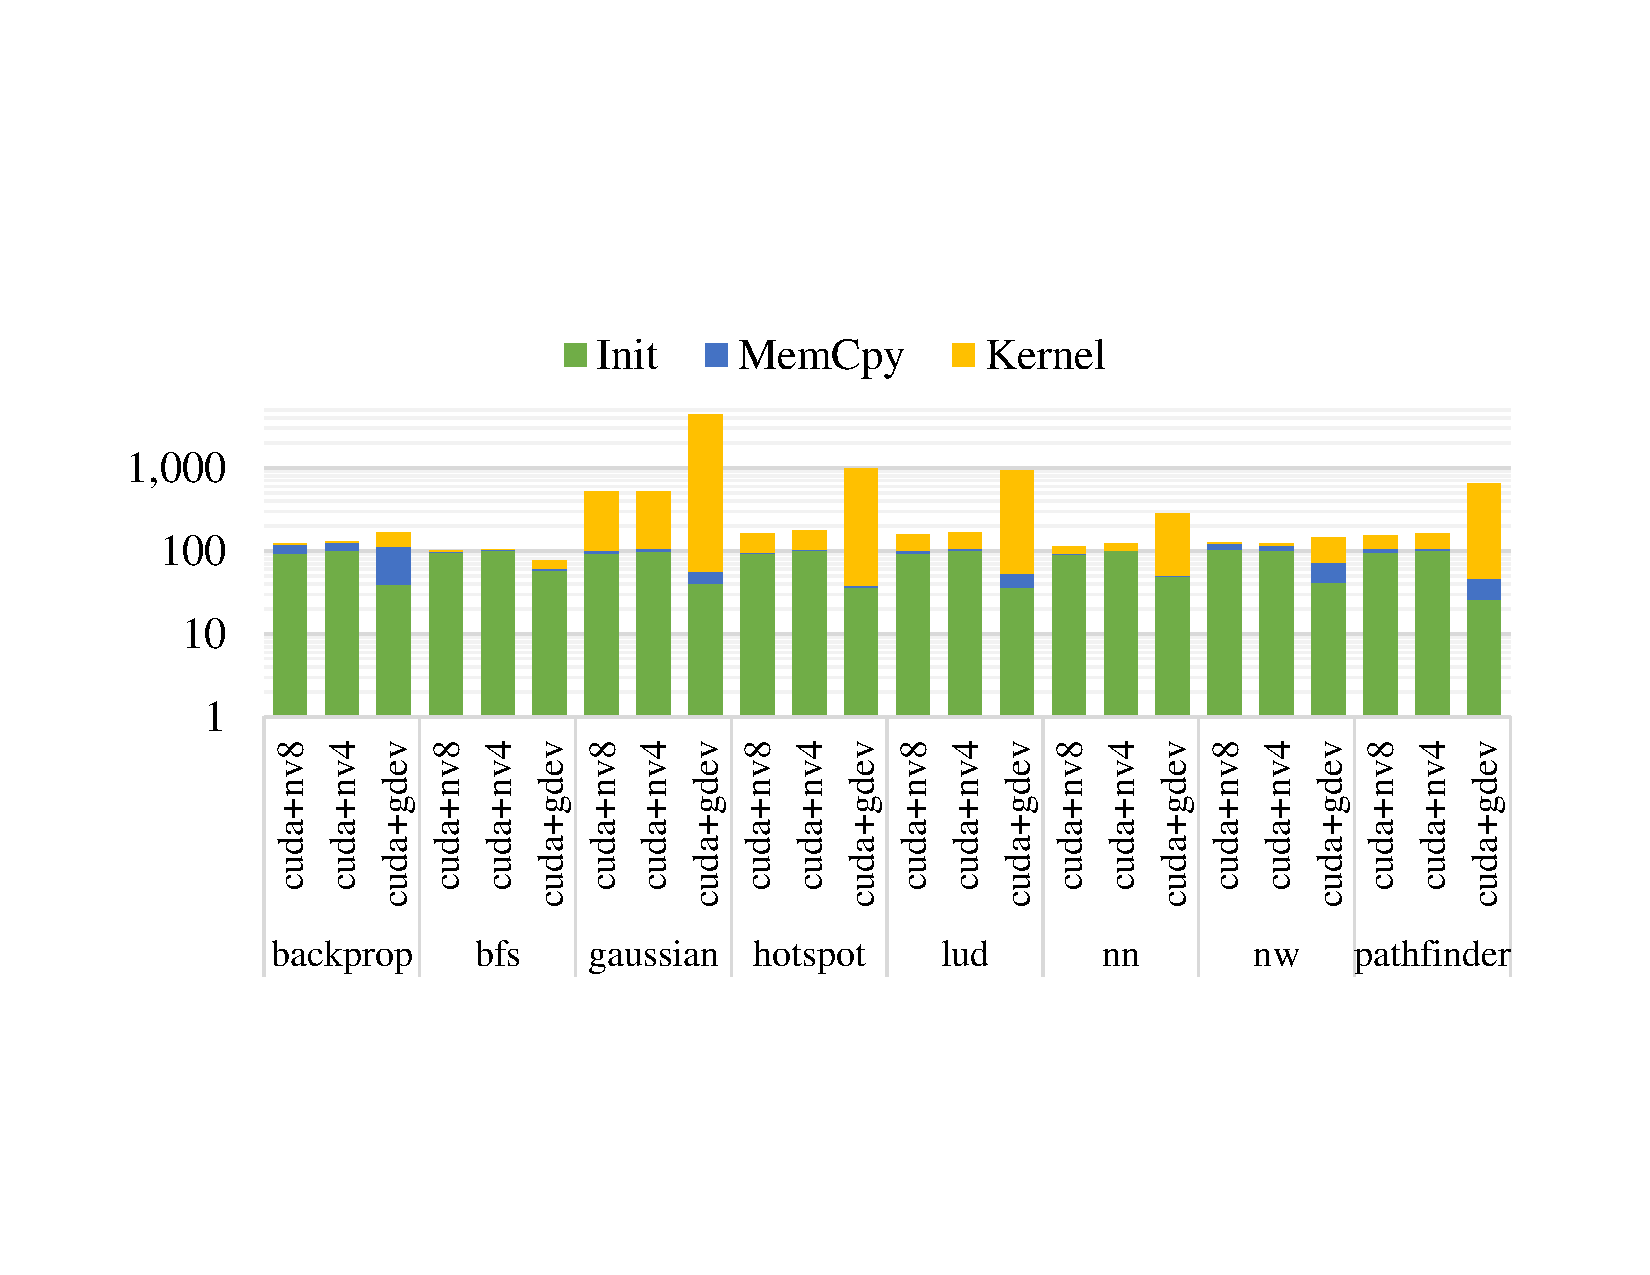
\includegraphics[width=1.1\linewidth,trim={2.3cm 5cm 2cm 5cm},clip]{data/basic/compiler.pdf}
%% 	\caption{{\footnotesize Runtime of benchmarks written in CUDA comparing impact of compiler version (NVCC 4.2 vs NVCC 8.0)
%% 		and runtime implementation (CUDA vs \texttt{gdev}).	Note that \texttt{gdev} depends on NVCC 4.2.}}
%% 	\label{fig_compiler} \end{figure}


%% Figure~\ref{fig_compiler} shows these results. When the NVIDIA stack is used,
%% the \texttt{nvcc} version has negligible impact, but there are important
%% differences introduced by \texttt{gdev}. While memory copy and kernel execution
%% times are often the same, \texttt{gdev} performs initialization more
%% quickly, but in some cases results in significantly longer kernel execution
%% times, e.g. \texttt{gaussian}, for which kernel time is over an order of
%% magnitude slower. To understand how runtime implementation can impact GPU side
%% execution time, recall that the front end CUDA compiler produces an IR (PTX)
%% which is finalized to the native ISA (SASS) by a JIT compiler \emph{in the
%% driver}. The PTX to SASS finalization in the NVIDIA Runtime is clearly better
%% optimized than the one used by \texttt{gdev} (implemented by the Nouveau
%% driver).

%% The harmonic mean delta between \texttt{gdev} and NVIDIA runtimes is X\%
%% and the distribution is bimodal. Consequently, controlling for variability
%% introduced by comparisons of designs that use it is difficult. Because
%% it remains an essentially open variable, we are careful to point out
%% scenarios in which it may introduce significant experimental noise.
%% \cjr{We need to sort this out. harmonic mean delta is around 1000\%
%% pretty consistently. Moving on while sorting this out with Hangchen.}
%% \hyu{Don't get the point of this paragraph.. If we don't normalize the runtime with
%% different baselines, why does this really matter?}

%The \texttt{Init} is faster in GDev because the runtime finishes part of the initialization work
%before application's main function starts.
%GDev has much more overheads than \cite{gdev}, probably because
%of the different settings of Xen and physical devices.
% \subsection{Compilation optimization}
% \label{sec_compilation}
% We use NVCC~4.2 to compile the CUDA kernel for GDev, while we use NVCC~8 in all other situations.
% To clarify the possible optimization brought by newer compiler and GPU driver, we compare the
% benchmarks' performance with CUDA toolkit 4.2 and 8.0.

\paragraphbe{Hardware Generations.} The performance improvements over the
span of generations between the Quadro 6000
%(on which most of the systems have a dependency)
and modern cards is substantial. To estimate the effect of this variable we
ran all benchmarks on both Quadro 6000 and a more recent GPU, Quadro P6000.
While overall execution times are improved substantially, and the ratio of
time spent on the host to time spent on the GPU changes as a result, the
relative speedups are uniform across all benchmarks. This suggests that the
trends that we observe on the Quadro 6000 still hold on newer hardware. We
re-iterate that software dependencies of the GPUvm baseline prevent us
from using more recent hardware. Our evaluation is performed on the newest
(several generations older) GPU hardware that all our systems can run on.
% but this finding suggests that our findings will continue to hold as
% virtualization systems catch up with current hardware generations.
% \cjr{Reasonable? I think we did something like this, didn't we? Or am
% I making it up?} \hyu{Reasonable. But shall we also mention the new GPU
% features that can improve the virtualization performance (e.g pagefault)?}

% !TeX root = ../dissertation.tex

\section{Evaluation}
\label{sec:trilliumeval}

% \begin{figure*}[!ht!!]
% 	\centering
% 	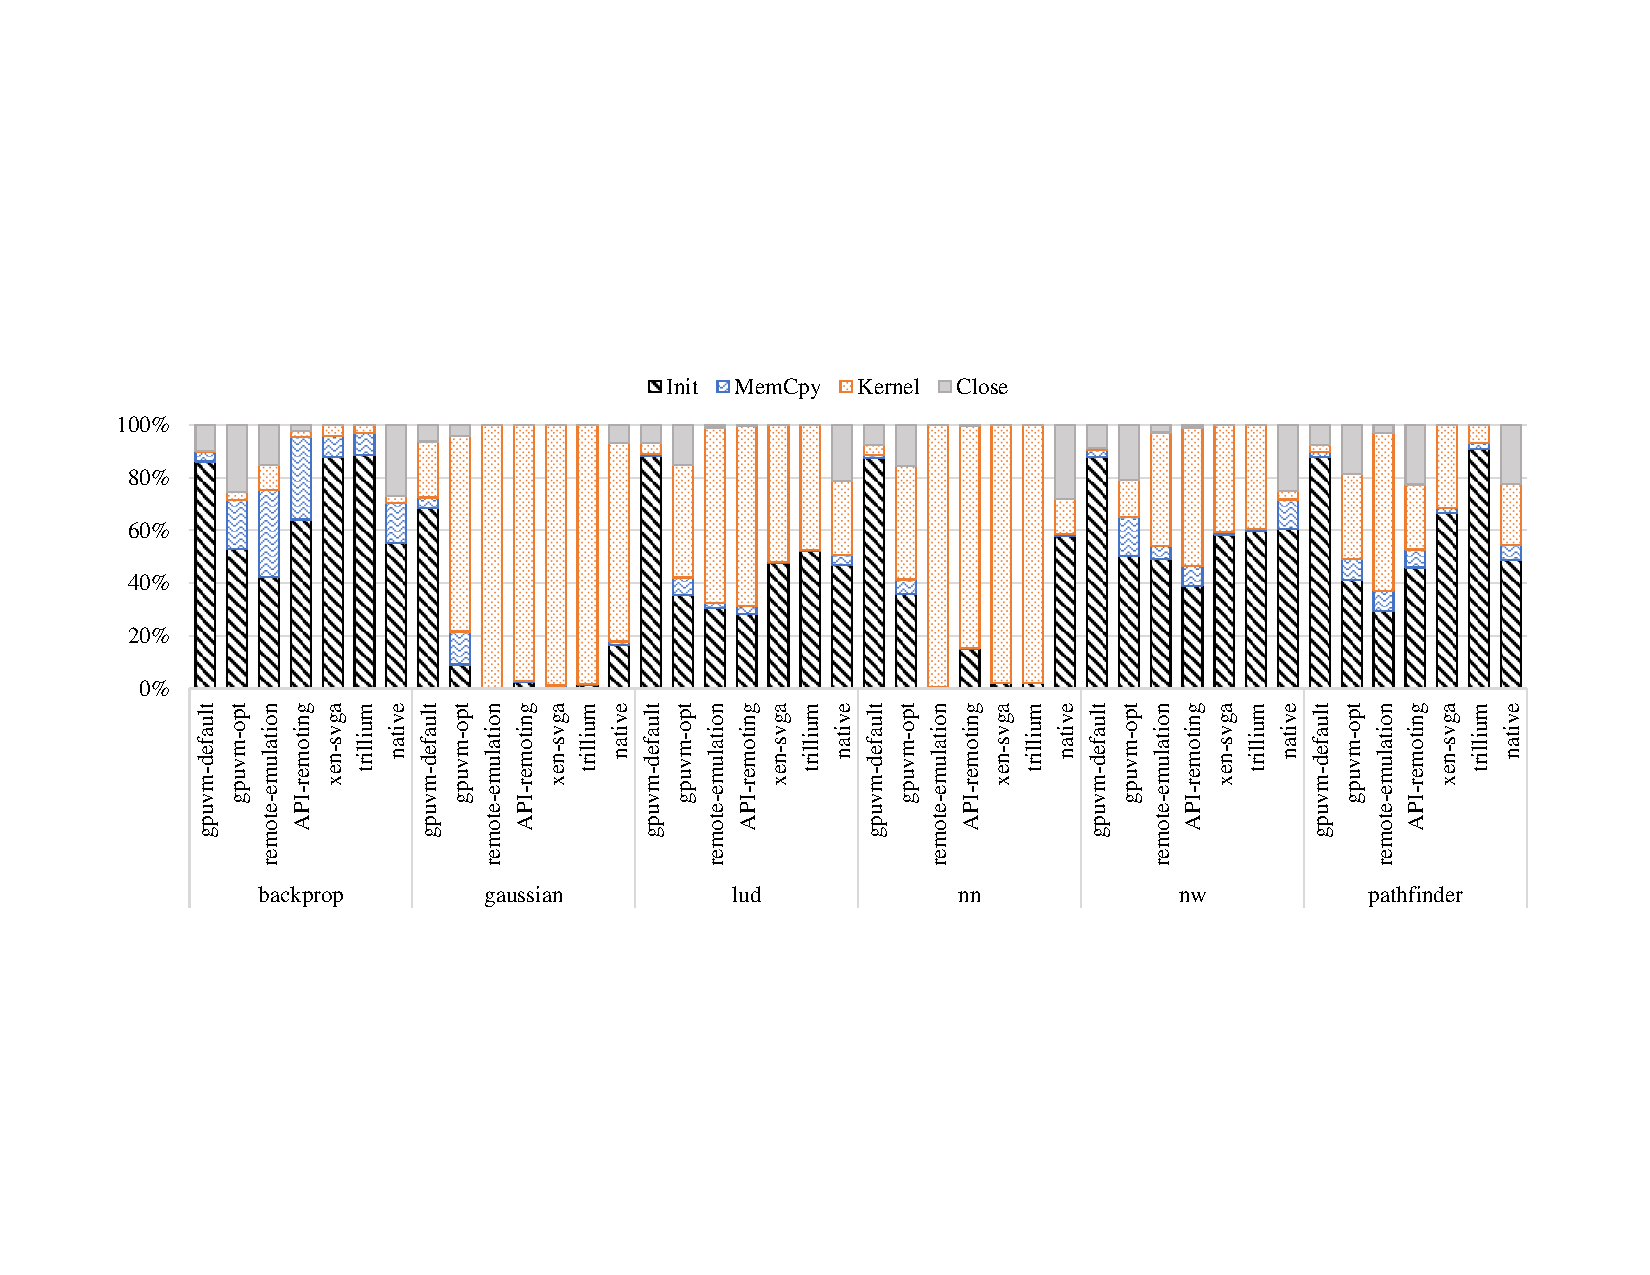
\includegraphics[width=.9\linewidth,trim={2cm 6cm 2cm 6cm},clip]{data/cross_product_breakdown_noRPC_OptInit.pdf}
% 	\caption{{\footnotesize Runtime breakdown of GPU benchmarks on virtualization prototypes.}}
% 	\label{fig_all_breakdown} \end{figure*}

We are interested in understanding the impact of a vISA on end-to-end performance, the effect of interposition frequency on performance, and the effectiveness of our proposed design, \Trillium.

\subsection{The impact of vISA choice}

%% \begin{figure}[!ht]
%% 	\centering
%% 	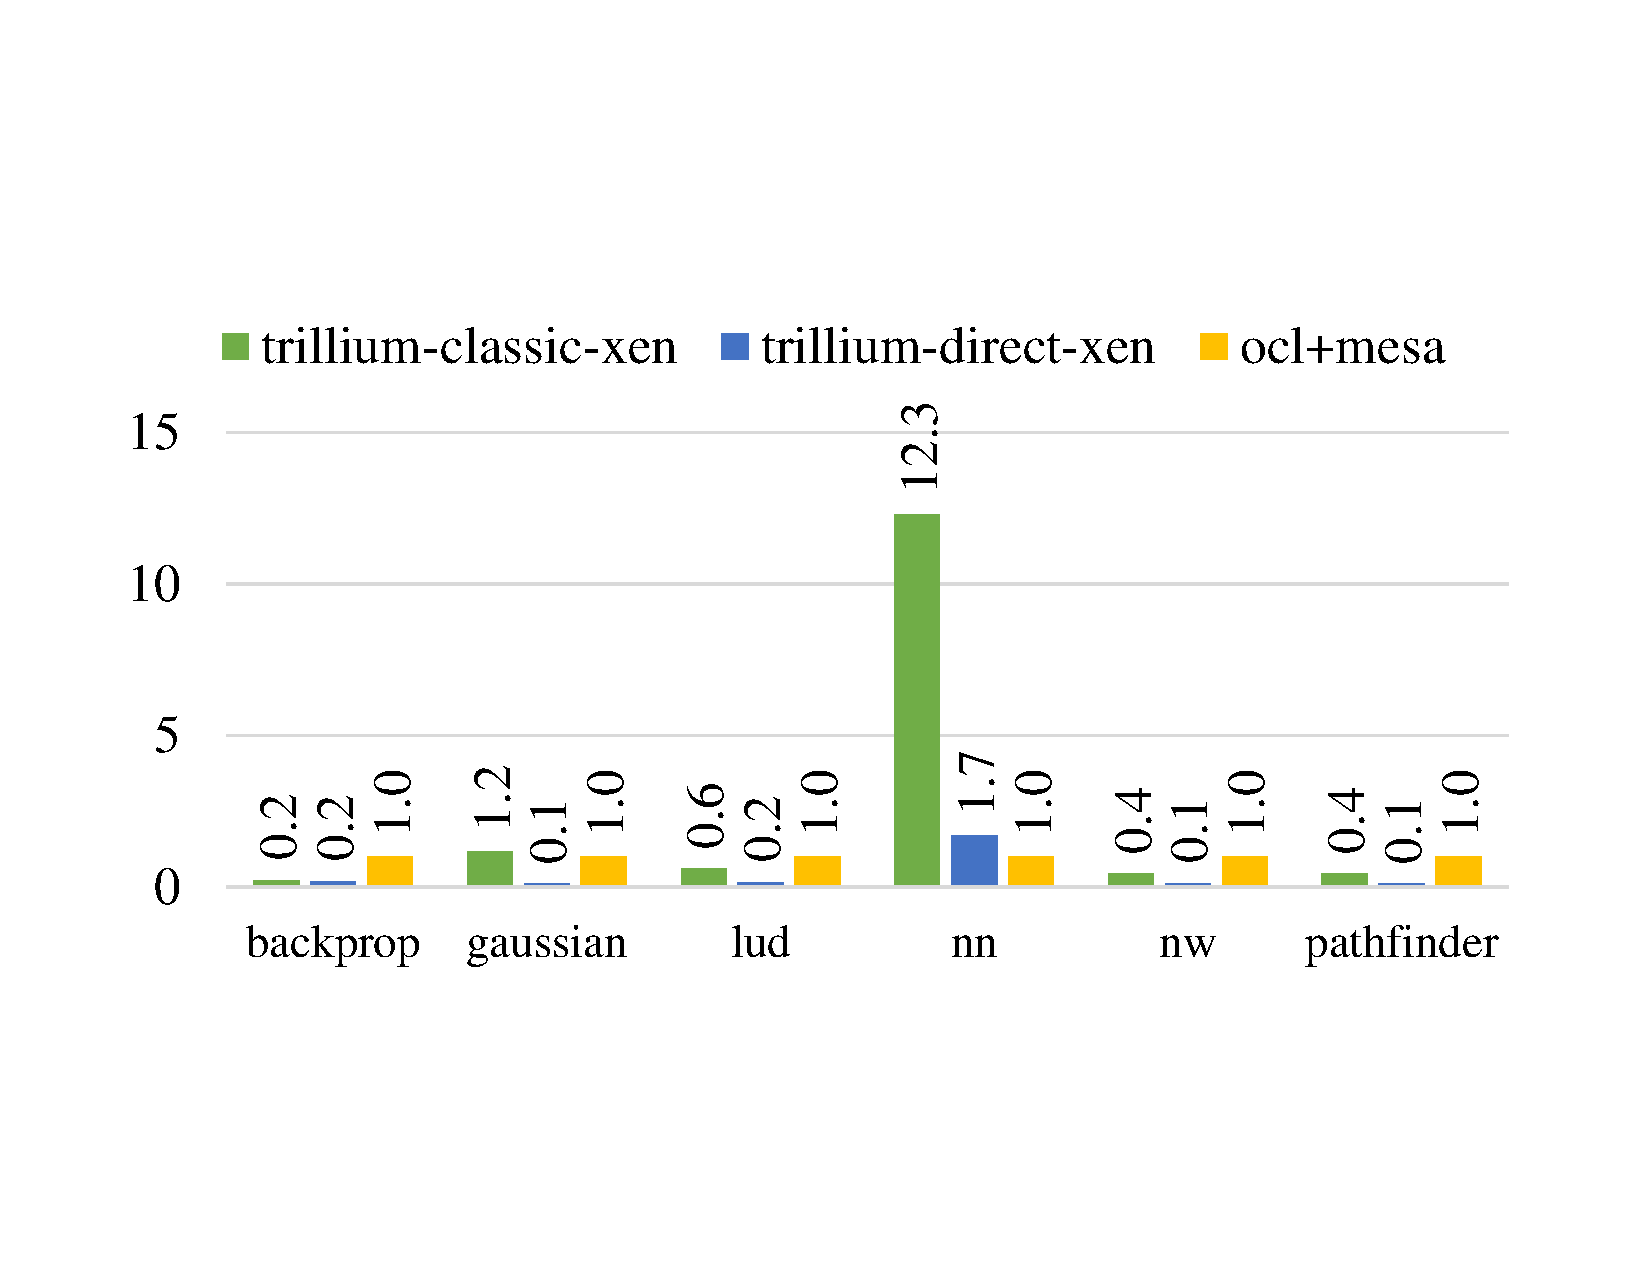
\includegraphics[width=\linewidth,trim={2.2cm 5cm 2.2cm 5.5cm},clip]{data/trillium/pipe_overhead_noRPC_OptInit.pdf}
%% 	\caption{{\footnotesize Overheads of the Trillium models with shadow pipe. \texttt{OpenCL+Mesa} is the baseline.}}
%% 	\label{fig_pipe_overhead} \end{figure}

%% \begin{figure}[!ht]
%% 	\centering
%% 	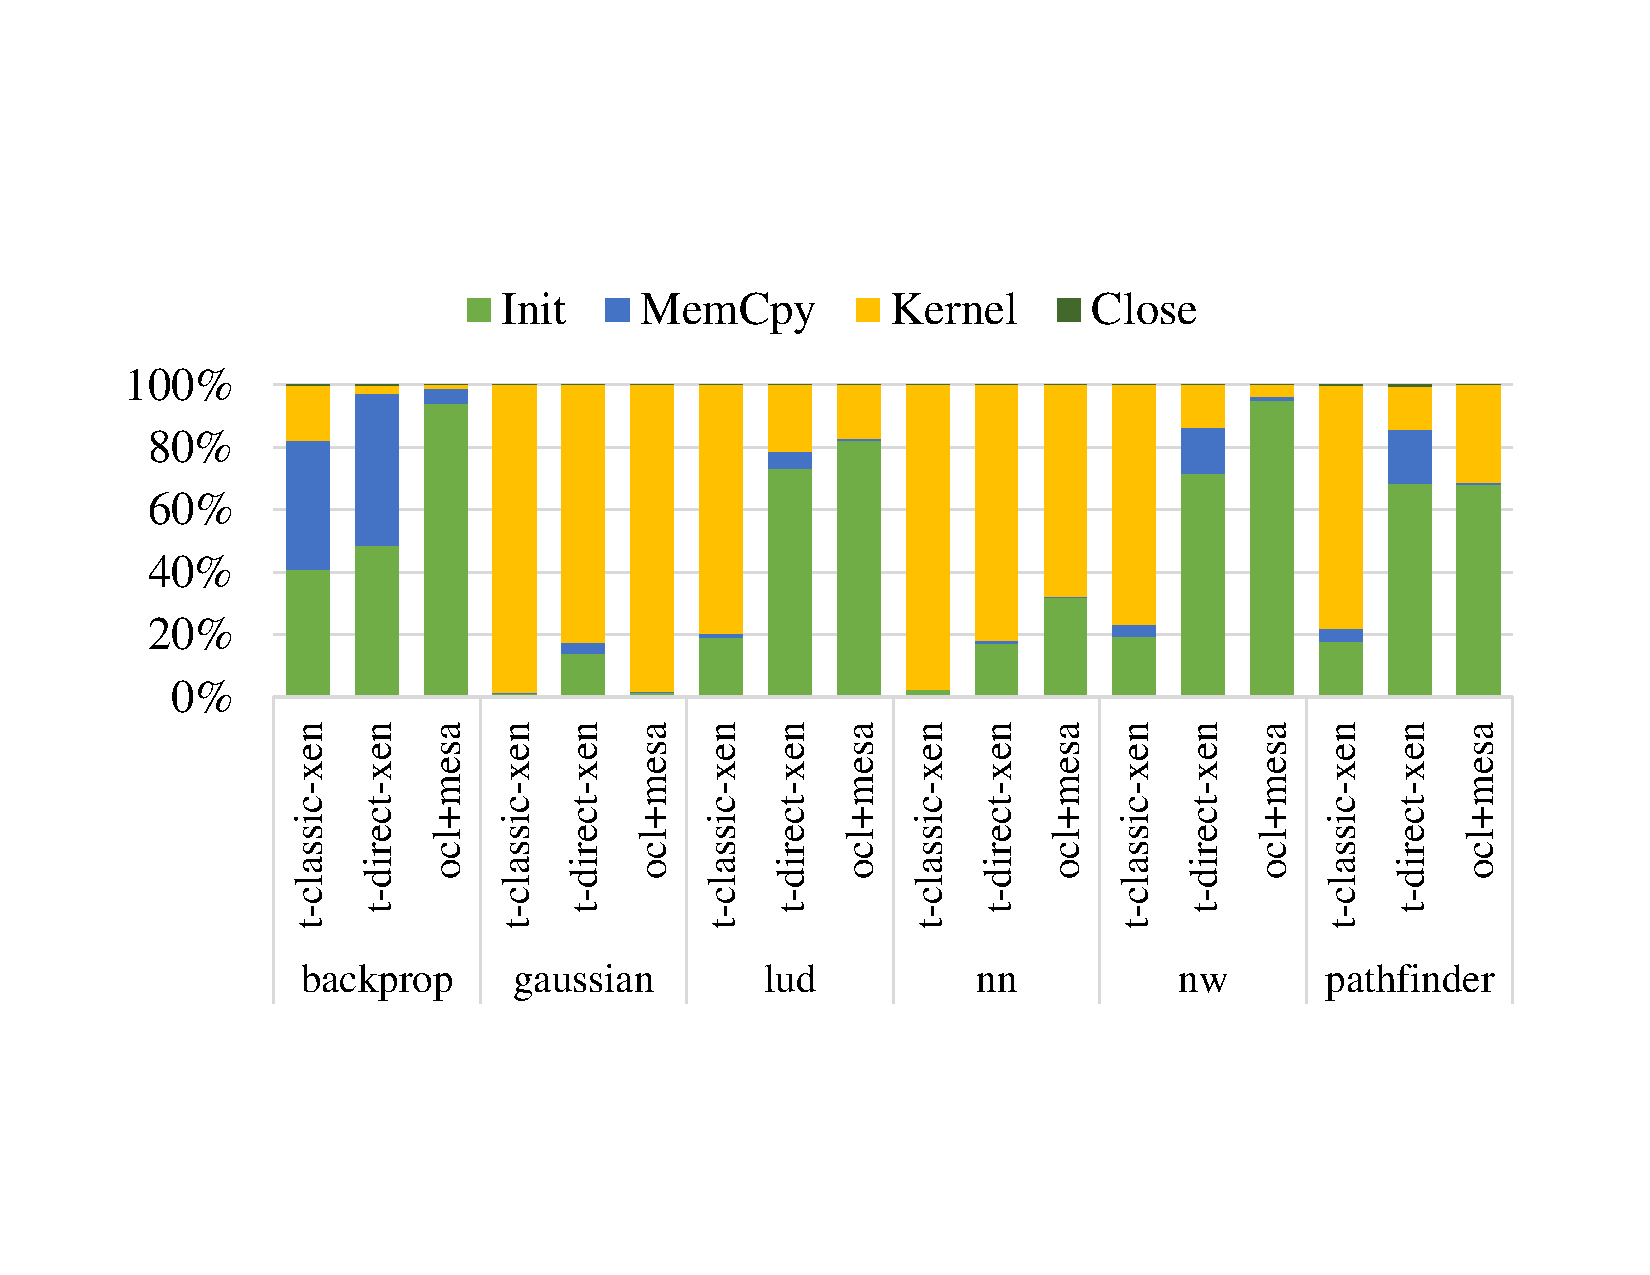
\includegraphics[width=\linewidth,trim={2.2cm 4.5cm 2.2cm 4.8cm},clip]{data/trillium/pipe_breakdown_noRPC_OptInit.pdf}
%% 	\caption{{\footnotesize Rumtime breakdown of the GPU benchmarks on the Trillium models with shadow pipe.}}
%% 	\label{fig_pipe_breakdown} \end{figure}

% The key difference between \Trillium-classic and \Trillium-direct is
% avoiding the use of a virtual instruction set in the guest.
% This eliminates a compiler transformation, but more importantly
% impacts
% these effects are visible, to put them in starker relief,
% the vendor-supplied compiler to be used under the virtualization layer
% (in this case the NVIDIA OpenCL stack), and for a design that produces
% LLVM in the guest, and finalizes that to NVIDIA SASS in the hypervisor.

%We re-iterate that our TGSI implementation is unoptimized
%and quantifying the performance loss attributable to that alone is difficult.

% \aak {I'm tempted to just remove the following. It doesn't really add anything to the paper.}
% We manually inspected the SASS binaries produced by the Nvidia and open source
% frameworks to understand the performance differences. While an in depth of
% analysis is beyond the scope of this paper, we make the following observations.

% \begin{compactitem}
% \item Both of the binaries benefit from common optimizations such as loop
% 	unrolling, and constant propagation, courtesy of LLVM.
% \item SASS code produced through the TGSI has substantially more convergence
% 	points (SYNC and SSY) instructions, which represent additional opportunity
% 	for control flow divergence.
% 	 % Table~\ref{tab:sassdiferences} presents the number of control flow instructions in the two binaries, as a proxy for diverging control flow.
% \item NVIDIA-produced SASS produces very different instruction sequences in
% 	several cases, e.g. XMAD (16bit Multiply Add) vs FFMA in TGSI (32-bit
% 	Fused Multipy Add). Our conjecture, in keeping with our hypothesis, is
% 	that the NVIDIA compiler has better information about which instructions
% 	more efficent on a particular architecture. It may be possible to
% 	reproduce some of these optimizations in the TGSI to SASS transformation,
% 	but since production of the TGSI code cannot rely on knowledge of the
% 	architecture, some optimizations may be impossible.
% \end{compactitem}
% \cjr{update me Amogh!}
% % !TeX root = ../dissertation.tex
\begin{table*}[h!]
\centering
% \footnotesize{
\begin{tabular}{@{}lllllllll@{}}
\toprule
           & \multicolumn{4}{l}{LLVM+PTXAS} & \multicolumn{4}{l}{Clover+Nouveua} \\ \midrule
           & SYNC    & SSY   & BRA   & BB   & SYNC     & SSY    & BRA    & BB    \\
bfs        & 0       & 0     & 15    & 12   & 8        & 4      & 5      & 18    \\
gaussian   & 0       & 0     & 23    & 18   & 6        & 3      & 3      & 9     \\
nn         & 0       & 0     & 9     & 7    & 0        & 0      & 0      & 4     \\
nw         & 10      & 5     & 18    & 23   & 8        & 4      & 8      & 18    \\
pathfinder & 9       & 5     & 18    & 23   & 12       & 6      & 7      & 32    \\
lud        & 31      & 13    & 67    & 76   & 20       & 10     & 14     & 35    \\ \bottomrule
\end{tabular}
% }
\caption{\footnotesize{Possible sources of performance differences between kernels generated using LLVM+PTXAS (comparable to NVCC) and Clover+Nouveau.}}
\label{tab:sassdiferences}
\end{table*}

% Table~\ref{tb_clover_slowdown} shows slowdowns of the Clover OpenCL runtime.\cjr{what is this  supposed to be?}
% \hyu{We wanted to factor out the impact of runtime. This table is not useful if we don't need to analyze the performance
% of Clover. It seems that we are only focusing on the Kernel time.}


\begin{figure*}[!ht!!]
	\centering
	% \includegraphics[width=.9\linewidth,trim={2cm 7.5cm 2cm 7cm},clip]{data/cross_product_overhead_noRPC_OptInit.pdf}
	\includegraphics[width=.9\linewidth,clip]{trillium/data/cross_product_overhead_noRPC_OptInit.pdf}
	\caption{{\footnotesize End-to-end execution times of benchmarks on virtualization prototypes, relative to end-to-end execution time on the NVIDIA CUDA runtime in a native setting.
			The gRPC transport overhead is removed from the reported measurements, which is up to 10\% of the total execution time for API remoting, and 40\% for \Trillium.}}
	\label{fig_all_overhead} \end{figure*}

\begin{figure}[!ht]
	\centering
	% ,trim={2.2cm 5cm 2.2cm 5.5cm},clip
	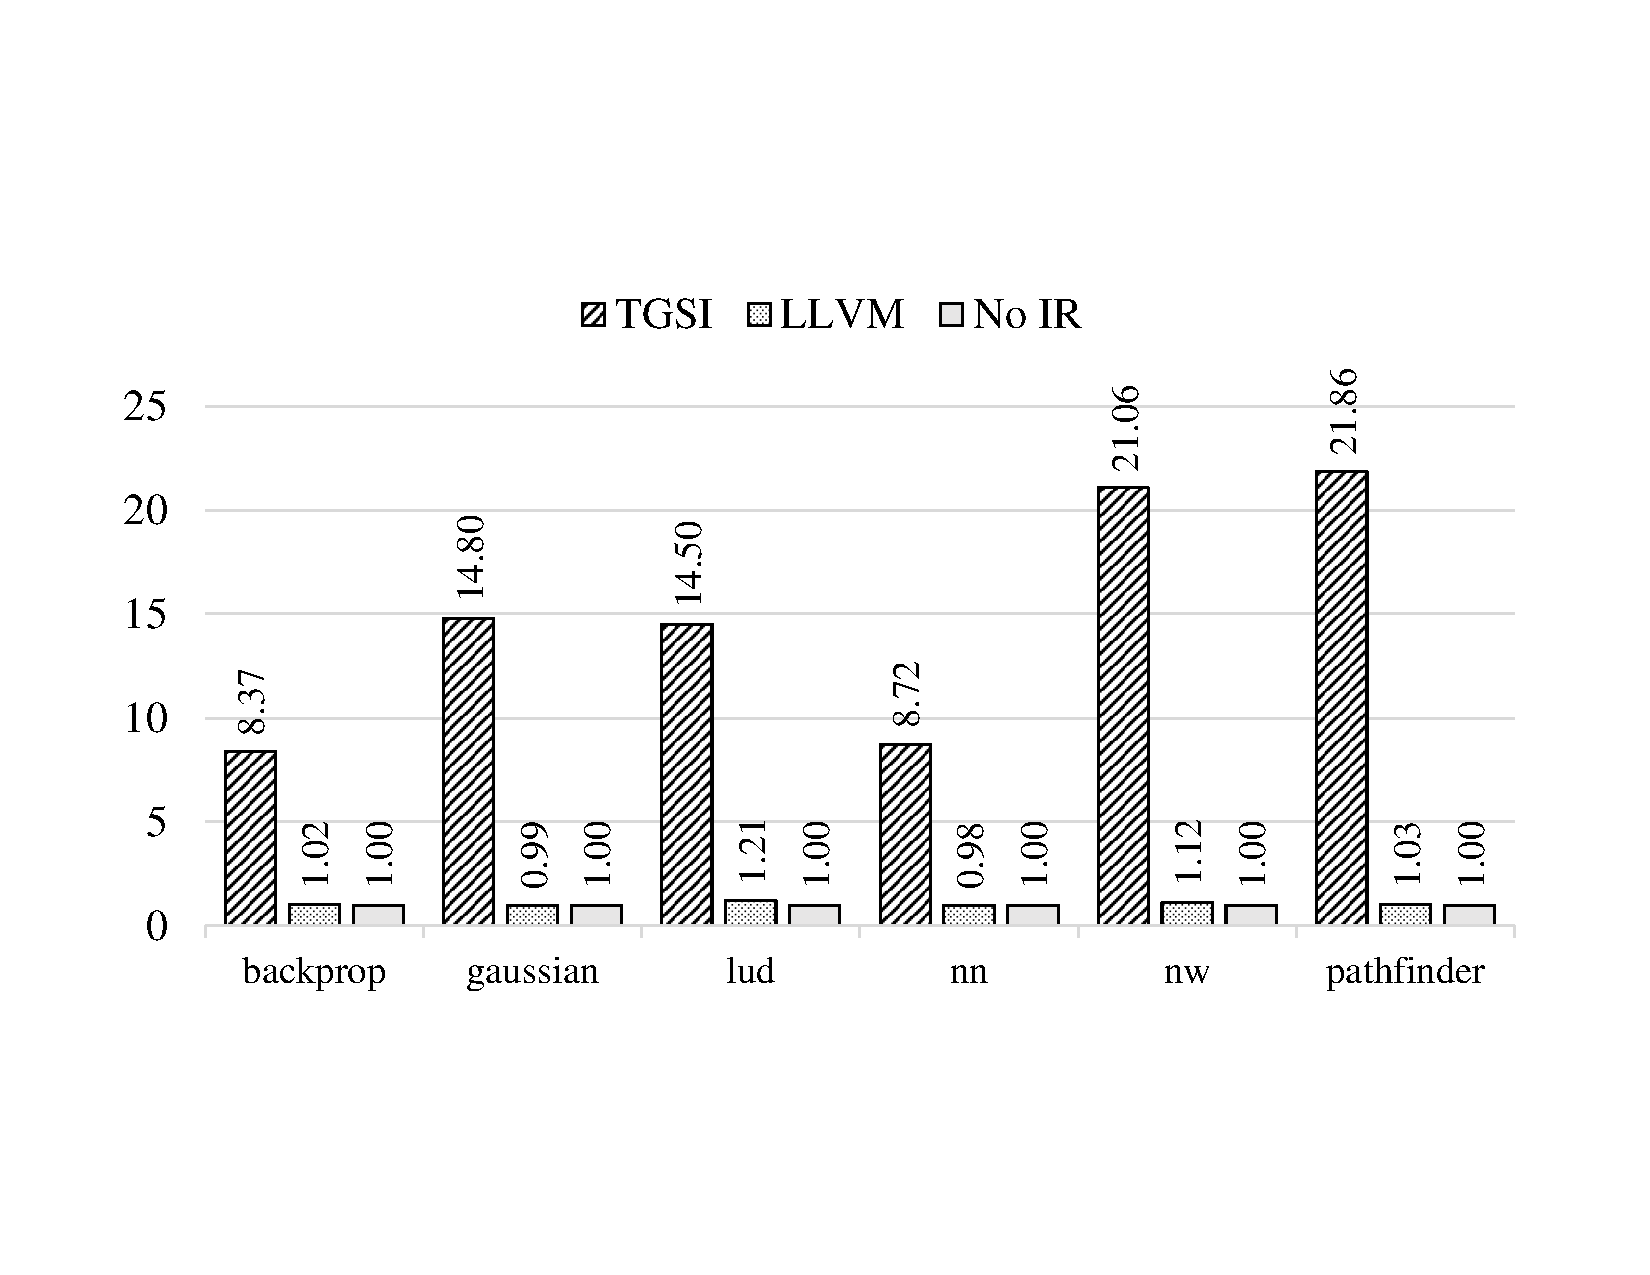
\includegraphics[width=.9\linewidth,trim={2cm 4.5cm 2cm 5cm},clip]{trillium/data/trillium/trillium_kernel.pdf}
	\caption{{\footnotesize Kernel execution slowdown due to virtual ISAs. TGSI: the LLVM TGSI back-end compiler used in \XenSVGA. LLVM: LLVM NVIDIA PTX (NVPTX) back-end used in \Trillium. No IR: native NVIDIA compiler.}}
	\label{fig_trillium_kernel}
\end{figure}

Deferring the compilation of front-end code to the host not only
eliminates redundant translations, and the need to have a compiler in the
guest driver,
 % that can translate supported compute frameworks to TGSI,
but also ensures that the compiler has a high-fidelity view of
the physical hardware. Typically, the execution/compilation framework is
extremely tightly coupled with the vISA used, making the choice of vISA even
more tenuous as it leads to the second order effect of having to rely on a
particular implementation of the compute framework (e.g., Mesa3D OpenCL vs NVIDIA OpenCL).
% This is especially significant given the nature of GPGPU computation.
%, instead ofhaving the option to use the best performing framework.

To understand the impact of the virtual ISA on the quality of the generated GPU code
% code that is ultimately run on the hardware,
we measured GPU execution time for NVIDIA SASS kernels generated in 3 ways:
a) using the Mesa3d OpenCL stack (OpenCL$\rightarrow{}$TGSI$\rightarrow{}$SASS),
b) using the LLVM OpenCL stack (OpenCL$\rightarrow{}$LLVM IR$\rightarrow{}$SASS),
and c) using the native NVIDIA OpenCL compiler (OpenCL$\rightarrow{}$SASS).
% , leaving out other overheads
% induced for virtualization, data, and device management.
These measurements are reported in Figure~\ref{fig_trillium_kernel}
relative to kernel execution time in a native setting.
% The Mesa3D OpenCL stack (Clover$+$Nouveau), which uses the TGSI
% ISA internally, is used to examine \XenSVGA and \Trillium.
%and by executing OpenCL code natively using the NVIDIA OpenCL framework.
%We were unable to to separate the execution/compilation framework
%from the ISA used, due their extremely tight coupling.


Code generated from TGSI IR is dramatically slower in all cases than code
generated by the NVIDIA OpenCL framework. We observe slowdowns of up to 22$
\times$, with a harmonic mean of 13$\times$ across the 6 benchmarks that were
optimized for evaluation.
% \hyu{Mention why pick 6?}
While we
predicted the basic trend these experiments show, we were surprised by the
magnitude of the difference. We found quality of the kernel generated by the
LLVM NVPTX compiler to be comparable to native, at least in terms of execution
time. This is unsurprising given recent efforts~\cite{gpucc} to optimize the
LLVM tool-chain for NVIDIA GPUs.

The \Trillium design uses LLVM IR as the common virtual ISA for GPGPU applications,
where necessary: OpenCL code is compiled to PTX using the LLVM NVPTX back-end in the guest,
and then finalized and executed in the host using the NVIDIA CUDA framework.

% SPIR-V has recently been adopted by the MESA3D community as an alternative to
% TGSI. SPIR-V is designed explicitly for expressing GPGPU primitives, and thus is likely
% to display better performance. However, our core conclusion still applies:
% vISAs introduced by the graphics stack are an unnecessary translation layer.

%(Control experiments show that choice of compute framework has negligible
%impact on the kernel execution time. See Section~\ref{sec:control})
% The data suggests that LLVM IR may be a suitable vISA as it enables GPU code
% whose quality is not substantially different from native execution.

\subsection{End-to-End}


We compare \Trillium against full-virtual (\gpuvmdef and \gpuvmopt),
API remoting (\apigpu and \apicpu) and para-virtual (\XenSVGA) systems.
\XenSVGA approximates an SVGA-like design in Xen (Mesa3D with TGSI). \Trillium
% is very similar, other than that it
bypasses translation from OpenCL to TGSI.
To characterize the behavior a full-virtual\-ization design, we measure
GPUvm~\cite{GPUvm} in its default configuration (worst case) shown as \gpuvmdef,
and in its fully optimized configuration, labeled \gpuvmopt.
% We additionally API remoting, both with GPU and CPU back-end.

%\aak{We need to reword this claim, because we aren't the closest to native performance. That claim sits firmly with api-remoting. However, we do much better than api-remoting on other aspects, and are thus a more complete virtualization mechanism in some sense.}
%\cjr{dispatched.}
% \hyu{Good point.}
% \aak{Also, we need to explain why we ran only 6 applications, given that we claimed that 10 benchmarks could be built by the compiler (in the implementation section. The reduction in number is because of the effort of porting applications to work on the API-forwarding we used to implement Trillium. We have to explain that.)}
% \hyu{Explanations in my head: 1. space limit; 2. these 6 are representitive. Strong enough?}
% \cjr{Not sure I'd buy space limit as the argument. Plus it's not really true right?}

Figure~\ref{fig_all_overhead} shows the end-to-end execution time (relative to
native GPU execution) for the six chosen benchmarks for all the systems evaluated. As
expected, traditional API remoting designs incur the lowest overhead, which is
achieved by giving up hypervisor interposition.
\Trillium fares well with best case performance
of just 1.1$\times$ over native, and within 3.6$\times$ at worst. \XenSVGA is
sensitive to the performance lost in GPU kernel code resulting from redundant
compilation through TGSI (which adds significant overheads as previously shown in
Figure~\ref{fig_trillium_kernel}). \gpuvmopt exhibits about 9.1$\times$ slowdown for
applications with short-lived kernels (e.g. Needleman-Wunsh algorithm); the
overhead can be as high as 15.2$\times$ when the workload has long-running
kernels (e.g. Gaussian Elimination).
% \hyu{May be good to analyze D/R/M categories' performance.}
% \aak{Agreed, but there doesn't seemt to be any correlation between D/R/M and Trillium's performance. I don't understand why the behaviour exhinbited is the way it is, and at this point, meh.}

We find that remoting calls intended to a CPU is uniformly more
performant than full-virtualization of the GPU, and sometimes performs just as well as (backprop)
or better than remoting to the GPU (1.6$\times$ faster for the bfs benchmark. The performance gain
from accelerating the bfs kernel on the GPU is severely dwarfed by the cost of initialization on
the GPU).
% \hyu{Analyze the reason? Maybe quote some part of Section VI-A?}
% \aak{Again I don't really have the patience go dig it up... Let's make sure we understand our data really well for Ava... This conference is meh as it is...}
% We do not suggest that GPGPU virtualization designers should use CPUs; instead,
% We make two observations about this situation:
GPGPU compute is only economical when it provides acceleration over the CPU;
if overheads make the CPU competitive, the profitability threshold has been crossed.
Further, the competitiveness of \apicpu suggests opportunity: systems could back a virtual
GPU with CPU if they can detect when it is profitable to do so.

% Application types can impact performance greatly.
% Note that for GPUvm, GPU kernel execution time did not differ significantly from other systems before ported to newer Ubuntu and Xen platform;
% The dramatic overheads on GPUvm are mostly attributable to the use of trap-based interposition on communication through memory-mapped command queues and/or MMIO.
%\XenSVGA delivers similar performance in general to the best-case full virtualization system.

% \subsection{Runtime Breakdown} \label{sec:breakdown}

% Benchmark applications operate in several different phases:
% initialization, data transfer, GPU kernel execution, and close/ teardown, each of responds differently to the different virtualization mechanisms. To illustrate this, we present the percentage of time spent in initialization, data transfer, GPU kernel execution, and close/teardown for each benchmark and system in Figure~\ref{fig_all_breakdown}.
% \aak{What is the point we're trying to make here? Too tired...}
% As noted earlier, the benchmarks can be classified into three categories: \textit{interposition-dominant} benchmarks (e.g. gaussian and nn) that see lower overheads from \Trillium
% \textit{interposition-rare} applications (e.g. backprop and pathfinder) which run a small number of long-running kernels, thereby suffering very little API-interposition overhead, and additionally benefit from the speedup in \texttt{Init} time (pre-initialized by remote server).
% \textit{moderate-interposition} applications (e.g. lud, nw) which invoke a
% moderate number of API calls, and therefore bear some interposition induced
% overhead.
% For interposition-dominant benchmarks, \XenSVGA performs really poorly because of the . \Trillium is efficient because that layer is bypassed and interposed APIs are batched.

% \subsection{Miscellanea}

%% \subsection{API remoting}

%% The major overheads of API remoting method are caused by RPC and data transfer. We applied widely-used Google
%% Protocol Buffers and XML-RPC to implement the RPC client (the one which runs the benchmarks) and server
%% (the one which actually executes the GPU commands). However, data transfer can be accomplished using shared memory rings~\cite{xen}
%% or remote direct memory access (RDMA), dramatically lowering these costs relative to our prototype.~\cjr{check this later. are we reporting these overheads?}
%% \hyu{We report the RPC time, but exclude the data transfer time.}
%% \hyu{The data makes less sense if we also exculde the RPC time; then there'll be trivial overheads. But our current RPC implementation is too naive, leading to non-trivial RPC overheads; this fails our trillium-pipe to outperform GPUvm-opt.}
%% \hyu{The best case is where we have an excellent RPC framework.}
%% \hyu{Data used to exclude trillium-classic-xen's RPC time: data/trillium/pipe.xlsx . We aren't able to exclude
%% 	the RPC overhead of trillium-direct-xen because we don't have a really running prototype.}


%% RPC number Table~\ref{tb:rpc_num}. \hyu{this table seems helpful.}

%% \begin{comment}
%% \begin{table*}[!th]
%% 	\centering
%% 	\begin{tabular}{l|r|r|r|r|r|r|}
%% 		\cline{2-7}
%% 		& \multicolumn{1}{l|}{backprop} & \multicolumn{1}{l|}{gaussian} & \multicolumn{1}{l|}{lud} & \multicolumn{1}{l|}{nn} & \multicolumn{1}{l|}{nw} & \multicolumn{1}{l|}{pathfinder} \\ \hline
%% 		\multicolumn{1}{|l|}{api-remoting} & 46 & 12,298 & 2,688 & 2,018 & 552 & 91 \\ \hline
%% 		\multicolumn{1}{|l|}{shadow-pipe} & 33 & 22,514 & 4,208 & 11,007 & 2,813 & 66 \\ \hline
%% 	\end{tabular}
%% 	\caption{\footnotesize{Number of RPCs sent in API remoting and Trillium models.}}
%% 	\label{tb:rpc_num}
%% \end{table*}

%% RPC overhead Table~\ref{tb:rpc_overhead_abs} and \ref{tb:rpc_overhead_relative} \hyu{may confuse the reader. RPC overhead
%% 	depends on the RPC number, RPC size, and RPC cost percentage also depends on the end-to-end time. E.g. RPC takes much higher portion in api-remoting gaussian and nn, because the kernel time is much shorter, and frequent clSetKernelArg API calls are
%% 	required.}
%% \begin{table*}[]
%% 	\centering
%% 	\begin{tabular}{l|r|r|r|r|r|r|}
%% 		\cline{2-7}
%% 		& \multicolumn{1}{l|}{backprop} & \multicolumn{1}{l|}{gaussian} & \multicolumn{1}{l|}{lud} & \multicolumn{1}{l|}{nn} & \multicolumn{1}{l|}{nw} & \multicolumn{1}{l|}{pathfinder} \\ \hline
%% 		\multicolumn{1}{|l|}{api-remoting} & 24.68 & 3,908.87 & 232.12 & 715.03 & 278.55 & 30.18 \\ \hline
%% 		\multicolumn{1}{|l|}{shadow-pipe} & 17.42 & 10812.96 & 2338.37 & 5319.76 & 1319.14 & 26.46 \\ \hline
%% 	\end{tabular}
%% 	\caption{\footnotesize{RPC overheads in API remoting and Trillium models (milliseconds)}}
%% 	\label{tb:rpc_overhead_abs}
%% \end{table*}

%% \begin{table*}[]
%% 	\centering
%% 	\begin{tabular}{l|r|r|r|r|r|r|}
%% 		\cline{2-7}
%% 		& \multicolumn{1}{l|}{backprop} & \multicolumn{1}{l|}{gaussian} & \multicolumn{1}{l|}{lud} & \multicolumn{1}{l|}{nn} & \multicolumn{1}{l|}{nw} & \multicolumn{1}{l|}{pathfinder} \\ \hline
%% 		\multicolumn{1}{|l|}{api-remoting} & 2.79\% & 81.20\% & 30.14\% & 77.97\% & 37.18\% & 5.25\% \\ \hline
%% 		\multicolumn{1}{|l|}{shadow-pipe} & 0.56\% & 58.92\% & 26.92\% & 57.33\% & 22.13\% & 0.64\% \\ \hline
%% 	\end{tabular}
%% 	\caption{\footnotesize{Percentages of the RPC cost in API remoting and Trillium models.}}
%% 	\label{tb:rpc_overhead_relative}
%% \end{table*}
%% \end{comment}

% !TeX root = ../dissertation.tex
\section{Conclusion}
\label{sec_con}

% Virtualizing GPGPUs is a balancing act: there is no clear winner; only a set
% of design points each offering a different trade-off of key virtualization
% properties. The \vframework framework enables clear reasoning about these trade-offs.
\Trillium represents a local optima in the GPGPU virtualization space---by decoupling device
virtualization from GPU ISA virtualization, it maintains the virtualization benefits of
a para-virtual system, while exhibiting the performance of a user-space remoting system.
% !TeX root = proposal.tex
\section{Hypervisor-mediated API-remoting}
\label{sec:ava}

Practical virtualization must support sharing and isolation under flexible
policy with minimal overhead. The structure of current accelerator stacks
makes this extremely difficult to achieve.
Accelerator stacks are \emph{silos} (Figure~\ref{fig:silo})
comprising proprietary layers communicating through memory mapped interfaces.
This opaque organization makes it \emph{impossible} to interpose intermediate
layers cleanly to form a virtualization boundary. Practically interposable
alternatives leave designers with a Hobson's choice between critical
virtualization properties such as interposition and compatibility.

\begin{figure}[!ht]
	\centering
	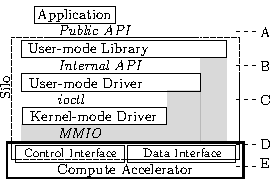
\includegraphics[width=.4\linewidth]{figures/silo.pdf}
	\caption{An accelerator silo.
		The public API and the interfaces with striped backgrounds are interposition candidates.
		All interfaces with backgrounds are proprietary and subject to change.
        }
	\label{fig:silo}
\end{figure}

We present \textsc{AvA}, a system that addresses the fundamental limitations
of existing accelerator virtualization techniques.
\textsc{AvA} combines API-agnostic para-virtual I/O stack components with a
Domain-Specific Language (DSL) and toolchain to automate construction
and deployment of guest libraries and API servers.
\textsc{AvA} uses an abstract para-virtual device to serve as a transport
endpoint for forwarding the public APIs of vendor-provided frameworks (e.g.
CUDA or TensorFlow). Unlike currently popular user-space API remoting
solutions~\cite{bitfusion,xaas,vmCUDA,rCUDA,cu2rcu}, \textsc{AvA} preserves
hypervisor-level resource management and strong isolation using a novel
technique called \emph{{{H}ypervisor {I}nterposed {R}emote {A}cceleration}}.
\textsc{AvA} forwards API calls over hypervisor-managed communication channels,
inserting automatically-generated resource management components between
traditional front- and back-ends
to enforce policies described in the DSL specification.
Critically, \emph{automation} from \textsc{AvA} enables hypervisors to keep up
with fast accelerator evolution: automatic generation of components minimizes
engineering effort.

\textsc{AvA} supports a broad range of currently-shipping compute accelerators:
We virtualized ten accelerators including NVIDIA and AMD GPUs, Google TPUs,
and Intel QuickAssist.
Virtualizing an API framework using \textsc{AvA} requires modest developer
effort:
a single developer virtualized OpenCL in a handful of days,
a stark contrast to the person-years of developer effort for VMware's SVGA II
or Bitfusion's FlexDirect~\cite{bitfusion}.
Experiments show that \textsc{AvA} provides near-native performance (e.g., 2.4\% slowdown for TensorFlow and 5.6\% for CUDA), enforces isolation and fair sharing across guests, and supports live migration.

The proposed chapter will make the following arguments:

\begin{itemize}[nosep,leftmargin=1em,labelwidth=*,align=left]
\item The chapter demonstrates feasibility of automatically constructed virtual accelerator support, showing that a single technique can deal with many architectures, APIs, versions, and policies.
\item We introduce {{H}ypervisor {I}nterposed {R}emote {A}cceleration} (HIRA) to enable hypervisor-enforced isolation and sharing policies unachievable with current SR-IOV and API remoting systems.
\item We utilize a novel DSL, \textsc{Lapis}, for describing API functions, resources, and policies to enable automatic construction of virtual stacks from native header files.
\item Our evaluation shows low developer effort, strong isolation, and good performance.
\end{itemize}

This chapter will draw from joint work with Hangchen Yu, Arthur Peters and Christopher J Rossbach. Part of this work was published as a workshop paper~\cite{ava-hotos}, and a longer paper is under submission. As with any big system building effort, it was a team effort.
% !TeX root = proposal.tex
\section{IEMTS --- A new accelerator virtualization taxonomy}
\label{sec:iemts}

Traditionally, virtualization designs have been taxonomized
according to the core techniques employed (e.g. emulation, full- or para-virtualization,
API remoting, etc.), and evaluated
in a property trade-off space comprising performance,
compatibility, interposition, and isolation. \emph{Isolation} ensures that mutually distrustful
guests cannot access each other's data or harm each other's performance. \emph{Compatibility},
characterizes how well a design preserves the freedom of
hardware and software components to evolve independently: e.g. changes in the hypervisor
should not force changes to guest software.
Virtualization provides an indirection layer between
logical and physical resources by \emph{interposing} a well-defined
interface. The quality of
interposition determines the nature of benefits (e.g. extent of consolidation) afforded by a
virtualized system~\cite{waldspurger12cacm}.

Virtualization techniques are well explored, yielding conventional
wisdom about their fundamental trade-offs. For example,
\emph{full virtualization} interposes the software-hardware interface
to provide a virtual view of the
underlying hardware. This enables guests to run unmodified OS and
application binaries, yielding high compatibility. However, hardware interfaces
for GPUs rely heavily on MMIO and communication through memory, which
necessitates page-fault-based interposition~\cite{tian2014full,
intel_kvmgt,kindratenko2009gpu,montella2012general} techniques that cripple
performance.
\emph{Para-virtual} designs export an abstract device to the guest,
but require hypervisor-specific drivers and runtime libraries in the
guest, trading compatibility for improved performance.
\emph{API remoting (or forwarding)}~\cite{gupta2009gvim, dowty2009gpu,
giunta2010gpgpu, shi2012vcuda} aggregates high-level API calls
issued in VMs, running them on the host or in a dedicated appliance VM.
This technique can provide near native performance because API calls
are infrequent, but has poor compatibility because it requires
changes in guest applications or libraries.

We argue that the current \emph{de facto} taxonomy and property trade-off space
are illustrative but not informative for GPUs:
there is a large body of research that has had little influence on practice.
First, Classifying virtualization designs as API-remoting vs. full vs.
para-virtual captures important concepts, and emergent properties compactly,
but doesn't explain their correlation to properties like performance.
Second, virtualization properties such as compatibility, isolation, and
interposition have highly context-dependent meaning and their relative value
to system designers can be hard to quantify.
Consider compatibility: there are many dimensions to compatibility (library,
hardware, OS, etc.), and each of those are commonly achieved by separate
technical, and non-technical means (e.g., TGSI is the common vISA for both the
VMware and GNU/Linux graphics stacks; this is \emph{not a lucky coincidence}).

We argue that practical design goals, such as providing a virtualization layer
with specific characteristics, get obscured when these properties are
considered as a set of constraints that must be preserved, without first
refining for context.
Further, production systems, such as VMware SVGA~\cite{dowty2009gpu},
compose multiple virtualization techniques in order to leverage the best
properties of each technique, especially in the presence of multiple
interfaces.

To enable a cleaner separation of concerns, we draw on the observation that
\textit{all} virtualization relies on encapsulation and interposition, and
note that a design can be clearly understood by identifying:
\begin{itemize}[nosep,leftmargin=1em,labelwidth=*,align=left]
\item the \textbf{I}nterface that is interposed,
\item the \textbf{E}nd-points (source and destination) the interposed event is transported between,
\item the \textbf{M}echanism used to interpose,
\item the \textbf{T}ransport mechanism used to communicate between endpoints,
\item the mechanisms used to \textbf{S}ynthesize or implement the desired functionality at the destination. We call this the \textbf{\texttt{IEMTS}} framework.
\end{itemize}

\begin{table*}[tt!]
\centering
\footnotesize
\resizebox{\textwidth}{!}{%
\begin{tabular}{@{}p{0.25\linewidth}|p{0.18\linewidth}|p{0.18\linewidth}|p{0.2\linewidth}|p{0.2\linewidth}@{}}
\toprule
\multirow{2}{*}{}         & \multirow{2}{*}{GPUvm} & \multicolumn{2}{c|}{VMware SVGA}             & \multirow{2}{*}{rCUDA} \\
                          &                        & Control Interface & GPU ABI             &                        \\ \midrule
Interposed Interface      & MMIO/BAR               & DirectX APIs      & Device ISA              & Userspace API          \\
Interposition Source      & Trap handler           & Guest driver/libs      & Guest Driver            & Guest Library           \\
Interposition Destination & Host driver            & Host framework        & Host Driver             & Host/Server Daemon     \\
Interposition Mechanism   & Trap                   & Guest library          & Compilation to vISA                    & Guest Library Shim     \\
Transport                 & Fault                  & Hypervisor FIFOs   & Hypervisor FIFOs    & RPC                    \\
Synthesis                 & Emulation              & Call host API     & Binary translation   & Call Server API        \\ \bottomrule
\end{tabular}
}
\caption{Comparing virtualization designs using the \texttt{IEMTS} framework.}
\label{tab:new-dims}
\end{table*}

\aak{Add discussion of the Table.}

% !TeX root = proposal.tex
\section{Proposed work --- vTask}
\label{sec:vTask}

The previous chapters in the proposed dissertation showed that
hypervisor-mediation API-remoting is the only effective mechanism for sharing
API-controlled compute devices among mutually distrustful tenants, e.g., in a
cloud computing environment. Virtualization vendors, such as VMware, have
begun adopting API-remoting based solutions for accelerator virtualization~\cite{bitfusion-acquisition}.

API-remoting works by interposing on API calls invoked by the application in
the guest OS, and executing them in a surrogate, the API-server, in the host.
Typically, API-servers are associated with a single API framework (for
modularity and failure isolation between APIs/accelerators, and in order to be
able to use remote resources) and each API-server is a surrogate for a single
guest (to preserve isolation between guests). Applications that use multiple
accelerator API frameworks will, therefore, be associated with multiple
API-servers, one per framework.

\begin{figure}[ht!]
\centering
\captionsetup{justification=centering,width=\linewidth}
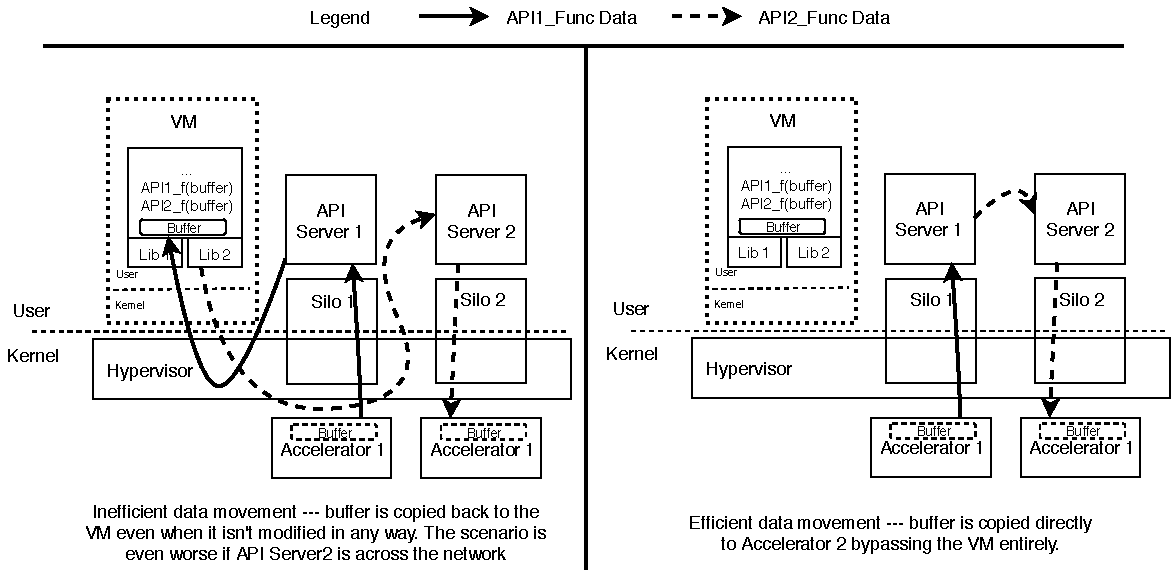
\includegraphics[width=\linewidth]{figures/vtask-overview.pdf}
\caption{Data processed by two API stacks must pass through the guest application}
\label{fig:overview}
\end{figure}

Under a typical API-remoting system, applications that pipeline disparate
accelerator frameworks are burdened with redundant data movement. All
inter-accelerator data movement must take place in the guest application as
that is where the accelerators are in the same logical address space.
Figure~\ref{fig:overview} illustrates this scenario: when an \emph{API-1}
function is invoked, associated data is copied from the
\emph{guest application} to \emph{API-server-1}, and then to \emph{Device-1}’s
memory. Once the function finishes executing on \emph{Device-1}, the result is
copied back to the \emph{guest application}. When a function from \emph{API-2}
is invoked, the same data (i.e., the output of the \emph{API-1 function}) is
copied from the \emph{guest application} to \emph{API-server-2} and then to
\emph{Device-2} to be processed.

In order to eliminate redundant data movement when an application uses
multiple accelerators via API-remoting, the hypervisor must track the data
passed to these API calls. The hypervisor must keep track of where the data
flowed from and to, the validity of different copies of the data (e.g., if the
data is modified on the accelerator, but hasn’t been copied back to the guest
application), and eliminate redundant data movement. As an example, if a guest
application were to invoke the \texttt{cudaMempyDtoH()} function to copy data
back from an Nvidia GPU, and then invoke the Intel QAT compression function
\texttt{cpaDCCompressData2()} on the same data without modifying it in any
way, the hypervisor should be able to detect this and elide the copying of
data to and from the guest application. Further optimization may also be
possible: peer-to-peer data copy between the devices if they are on the same
machine, or by directly copying the data from the first API-server on one
remote machine to the second API-server on another remote machine.

We propose to build vTask, an application-transparent data orchestration
system that optimizes data movement among accelerators virtualized via
API-remoting. vTask will leverage information from API
annotations~\cite{ava-hotos} to track data buffers across the guest
application, the API-servers servicing API calls made by the guest, and the
accelerator hardware. vTask will optimize data movement across these
components while ensuring that a coherent view of the data buffer is presented
to anyone attempting to read the data. Ideally, vTask will require no changes
to the guest application or  extra annotations of any kind from the
application programmer. We hypothesize that annotations provided to virtualize
the API (by the device or virtualization vendor) will be sufficient to infer
the semantics of the data buffers managed.

We will prototype vTask in AvA, a state-of-the-art para-virtual API-remoting
system for KVM. vTask will rely on device-side buffer allocation and
deallocation API calls, and special annotations provided by LAPIS, AvA’s API
description language, to determine buffer lifetime. Further, vTask will
implement a simple MESI-style coherence protocol to track spatial validity of
data (i.e., to track where the latest data is present). vTask will leverage
optimizations such as shared memory, Unified Virtual Memory, and PCIe
Peer-to-Peer (P2P) data transfer where available, but does not make
assumptions about their universal availability.

With vTask, AvA will be able to handle data movement between both local and
remote devices. When API-remoting to a remote system, the devices used by the
guest application may be present on separate machines. We hypothesize that
vTask will be able to eliminate costly data transfers over the network by
adhering to the principle of lazy loading wherever possible, i.e., data is not
moved until a demand fault occurs.

\aak{needed: a deeper explanation of design (breaking it down into the pieces that need to be built along with an estimation of how long each will take), a better evaluation strategy (with applications that we intend to run and how the machines will be setup, etc.)}

% !TeX root = proposal.tex
\section{Plan of Work}
\begin{table}[htp!]
\centering
\begin{tabular}{ll}
\toprule
Task 											& Deadline \\
\midrule
Dissertation proposal and oral exam				& Nov. 2019 \\
Implement vTask in AvA (submit to ATC'20) 		& 15 Jan. 2020 \\
Dissertation draft to committee					& 1 Mar. 2020 \\
Dissertation defense							& late Mar. 2020 \\
Submit dissertation to graduate school 			& 12 Apr. 2020 \\
\bottomrule
\end{tabular}
\caption{Proposed timeline.}
\label{tab:timeline}
\end{table}
% !TeX root = proposal.tex
\section{Related Work}
\label{sec:related}

Virtualization has such a long and storied history that Attempting to capture
the entire story is an exercise in futility. The introduction~\ref{sec:intro}
captures the history of CPU virtualization in broad strokes. This section then
focuses on a major theme of the proposed dissertation:
accelerator virtualization.

Accelerating specific computation is not a new idea---support for specialized
computation is extremely commonplace in CPUs (e.g., Floating Point Units
(FPU), Vector Processing Units). These specialized compute units are
typically exposed to the programmer as extensions to the Instruction Set
Architecture (ISA). Virtualizing these specialized compute units, therefore,
is no different from virtualizing the rest of the CPU and ISA virtulaization
is well explored~\cite{cp40,vm370,popek-goldberg,bugnion-disco,
bugnion-nieh-tsafrir,bugnion-workstation}.

Processors specialized for complex computational tasks, such as graphical
rendering, largely evolved as discrete devices separate from the CPU (although
some CPUs do integrate GPUs). These devices are not typically integrated into
the CPU ISA; instead, they appear to system software as I/O devices with
memory-mapped command-queues and I/O registers. I/O virtualization is well
understood~\cite{waldspurger12cacm,paradice,Kuperman_undated-io,Sig2010-ml,
zeng2013improved,abramson2006intel}, but these techniques aren't enough to
virtualize programmable accelerators. Although programmable accelerators look
like I/O devices, they are also general computing platforms, i.e., they load
binaries, have their own memory, and are typically exposed to the application
programmer via an API.

\subsection{GPU Virtualization}

% !TeX root = proposal.tex
\def\libnomod{lib unmod\xspace}
\def\osnomod{OS unmod\xspace}
\def\sharing{sharing\xspace}
\def\isolation{isolation\xspace}
\def\scheduling{sched. policy\xspace}
\def\perf{performance\xspace}
\def\libflex{lib-compat\xspace}
\def\hwflex{hw-compat\xspace}
\def\mobility{migration\xspace}
\def\gfx{graphics\xspace}
\def\gpgpu{GPGPU\xspace}
\def\id{I/D}
\def\discrete{\emph{D}}
\def\integrated{\emph{I}}
% \def\poor{--}
% \def\good{+}
% \def\ok{+/-}
% \def\verygood{++}
% \def\verybad{-- --}
\def\poor{\textbf{poor}\xspace}
\def\good{\textbf{good}\xspace}
\def\ok{\textbf{ok}\xspace}
\def\verygood{\textbf{excellent}\xspace}
\def\verybad{\textbf{bad}\xspace}
%\def\chk{$\times$}
\def\chk{\checkmark}
\def\cross{$\times$\xspace}
\def\gr{\cellcolor[gray]{0.9}}
\def\redc{\cellcolor[gray]{0.4}}
\def\bluec{\cellcolor[gray]{0.1}}

%\newcommand{\mc}[2]{\multicolumn{#1}{c}{#2}}
\definecolor{Gray}{gray}{0.6}
\definecolor{LightCyan}{rgb}{0.88,1,1}
%\newcolumntype{a}{>{\columncolor{Gray}}c}
\def\FV{\textbf{FV}}
\def\PT{\textbf{PT}}
\def\PV{\textbf{PV}}
\def\APIR{\textbf{API-R}}
\def\unmodlib{\textbf{UL}}
\def\unmodos{\textbf{UOS}}
\def\safe{\textbf{I}}
\def\fair{\textbf{F}}
\def\mob{\textbf{M}}

\setlength{\aboverulesep}{0pt}
\setlength{\belowrulesep}{0pt}

\begin{table*}[ht!]
\vspace*{2em}
\centering
\footnotesize{
\resizebox{\textwidth}{!}{
\begin{tabular}{r|l|c|c|c|c|c|c|c|c|c|c|c|c|c|c|c|}
%\hline
\T\B {\textbf{Technique}}       &
\T\B {\textbf{System}}          &
\rot{\textbf{\libnomod}}        &
\rot{\textbf{\osnomod}}         &
\rot{\textbf{\libflex}}         &
\rot{\textbf{\hwflex}}          &
\rot{\textbf{\sharing}}         &
\rot{\textbf{\isolation}}       &
\rot{\textbf{\mobility}}        &
\rot{\textbf{\parbox{4cm}{sched. \\policy}\xspace}}      &
\rot{\textbf{\gfx}}             &
\rot{\textbf{\gpgpu}}           &
\rot{\textbf{\id}}              &
\rot{\textbf{benchmark}}        &
\rot{\textbf{slowdown}}         &
\rot{\textbf{\parbox{4cm}{native\\speedup}}}    &
\rot{\textbf{\parbox{4cm}{virtual\\speedup}}}
\\   \hline

\T\B \multirow{2}{*}{\textbf{Full-virtual}}     &
     \T\B \textbf{GPUvm~\cite{GPUvm}}           &
     \T\B \chk                                  &  % unmodified guest libraries
     \T\B                                       &  % unmodified guest OS
     \T\B \chk                                  &  % lib-compatibility
     \T\B                                       &  % hw-compatibility
     \T\B \chk                                  &  % cross-VM sharing
     \T\B \chk                                  &  % cross-VM isolation
                                                &  % VM migration
     \T\B XC, BAND                              &  % fairness
                                                &  % graphics support
     \T\B \chk                                  &  % GPGPU support
     \T\B \discrete                             &  % integrated-discrete
     \T\B Rodinia                               &  % benchmark
     \T\B 141$\times$                           &  % base slowdown
     \T\B 11.4$\times$                          &  % native speedup
     \T\B {\textcolor{red}{0.08$\times$}}          % virtualized speedup
     \\ \cline{2-17}
                                                &
     \T\B \textbf{gVirt~\cite{gVirt}}           &
     \T\B \chk                                  &  % unmodified guest libraries
     \T\B                                       &  % unmodified guest OS
     \T\B \chk                                  &  % compatibility
     \T\B                                       &  % compatibility
     \T\B \chk                                  &  % cross-VM sharing
     \T\B \chk                                  &  % cross-VM isolation
     \T\B \chk                                  &  % VM migration
     \T\B QoS                                   &  % fairness
     \T\B \chk                                  &  % graphics support
     \T\B                                       &  % GPGPU support
     \T\B \integrated                           &  % integrated-discrete
     \T\B 2D~\cite{phoronix}, 3D~\cite{cairoperf}& % benchmark
     \T\B 1.6$\times$                           &  % base slowdown
     \T\B N/A                                   &  % native speedup
     \T\B N/A                                      % virtualized speedup
     \\ \hline

\T\B \textbf{PCIe Pass-thru}                    &
     \T\B \textbf{AWS GPU~\cite{amazongpu}}     &
     \T\B \chk                                  & % unmodified guest lib
     \T\B \chk                                  & % unmodified guest OS
     \T\B \cellcolor{gray!25}                   & % compatibility
     \T\B \cellcolor{gray!25}                   & % compatibility
     \T\B \cellcolor{gray!25}                   & % sharing
     \T\B \cellcolor{gray!25}                   & % isolation
     \T\B \cellcolor{gray!25}                   & % mobility
     \T\B \cellcolor{gray!25}                   & % fairness
     \T\B \chk                                  & % graphics
     \T\B \chk                                  &  % GPGPU support
     \T\B \discrete                             &  % integrated-discrete
     \T\B Any                                   &  % benchmark
     \T\B 1$\times$                             &  % base slowdown
     \T\B \cellcolor{gray!25}                   &  % natice speedup
     \T\B \cellcolor{gray!25}                      % virtualized speedup
     \\ \hline

\T\B \multirow{4}{*}{\bf API remoting}          &
     \T\B {\bf GViM~\cite{gupta2009gvim}}       &
     \T\B                                       &  % unmodified guest libraries
     \T\B                                       &  % unmodified guest OS
     \T\B                                       &  % lib-compatibility
     \T\B \chk                                  &  % hw-compatibility
     \T\B \chk                                  &  % cross-VM sharing
     \T\B \chk                                  &  % cross-VM isolation
                                                &  % VM migration
     \T\B RR, XC                                &  % fairness
                                                &  % graphics support
     \T\B \chk                                  &  % GPGPU support
     \T\B \discrete                             &  % integrated-discrete
     \T\B CUDA 1.1 SDK                          &  % benchmark
     \T\B 1.16$\times$                          &  % base slowdown
     \T\B 22$\times$                            &  % native speedup
     \T\B {\textcolor{blue}{19$\times$}}           % virtualized speedup
     \\ \cline{2-17}


                                                &
     \T\B {\bf gVirtuS~\cite{gVirtuS}}          &
     \T\B                                       &  % unmodified guest libraries
     \T\B                                       &  % unmodified guest OS
     \T\B                                       &  % lib-compatibility
     \T\B \chk                                  &  % hw-compatibility
     \T\B \chk                                  &  % cross-VM sharing
     \T\B \chk                                  &  % cross-VM isolation
                                                &  % VM migration
     \T\B RR                                    &  % fairness
                                                &  % graphics support
     \T\B \chk                                  &  % GPGPU support
     \T\B \discrete                             &  % integrated-discrete
     \T\B CUDA 2.3 MM                           &  % benchmark
     \T\B 3.1$\times$                           &  % base slowdown
     \T\B 11.1$\times$                          &  % native speedup
%     \T\B 3.6$\times$                              % virtualized speedup
     \T\B {\textcolor{blue}{3.6$\times$}}          % virtualized speedup
     \\ \cline{2-17}

                                                &
     \T\B \T\B {\bf vCUDA~\cite{shi2012vcuda}}         &
     \T\B                                       &  % unmodified guest libraries
     \T\B \chk                                  &  % unmodified guest OS
     \T\B                                       &  % lib-compatibility
     \T\B \chk                                  &  % hw-compatibility
     \T\B                                       &  % cross-VM sharing
     \T\B                                       &  % cross-VM isolation
     \T\B \chk                                  &  % VM migration
     \T\B HW                                    &  % fairness
                                                &  % graphics support
     \T\B \chk                                  &  % GPGPU support
     \T\B \discrete                             &  % integrated-discrete
     \T\B CUDA 4.0 SDK                          &  % benchmark
     \T\B 1.91$\times$                          &  % base slowdown
     \T\B 6$\times$                            &  % native speedup
     \T\B {\textcolor{blue}{3.1$\times$}}          % virtualized speedup
     \\ \cline{2-17}

                                                &
     \T\B {\bf vmCUDA~\cite{vmCUDA}}            &
     \T\B                                       &  % unmodified guest libraries
     \T\B \chk                                  &  % unmodified guest OS
     \T\B                                       &  % lib-compatibility
     \T\B \chk                                  &  % hw-compatibility
     \T\B \chk                                  &  % cross-VM sharing
     \T\B                                       &  % cross-VM isolation
     \T\B                                       &  % VM migration
     \T\B HW                                    &  % fairness
                                                &  % graphics support
     \T\B \chk                                  &  % GPGPU support
     \T\B \discrete                             &  % integrated-discrete
     \T\B CUDA 5.0 SDK                          &  % benchmark
     \T\B 1.04$\times$                          &  % base slowdown
     \T\B 33$\times$                            &  % native speedup
     \T\B {\textcolor{blue}{31.7$\times$}}         % virtualized speedup
     \\ \hline


\T\B \multirow{4}{*}{\bf \shortstack[r]{Distributed\\API remoting}}  &
    \T\B {\bf rCUDA~\cite{rCUDA, rCUDAnew}}     &
     \T\B                                       &  % unmodified guest libraries
     \T\B \chk                                  &  % unmodified guest OS
     \T\B                                       &  % lib-compatibility
     \T\B \chk                                  &  % hw-compatibility
     \T\B \chk                                  &  % cross-VM sharing
     \T\B \chk                                  &  % cross-VM isolation
     \T\B                                       &  % VM migration
     \T\B RR                                    &  % fairness
                                                &  % graphics support
     \T\B \chk                                  &  % GPGPU support
     \T\B \discrete                             &  % integrated-discrete
     \T\B CUDA 3.1 SDK                          &  % benchmark
     \T\B 1.83$\times$                          &  % base slowdown
     \T\B 49.8$\times$                          &  % native speedup
     \T\B {\textcolor{blue}{27.2$\times$}}         % virtualized speedup
     \\ \cmidrule{2-17}

                                                &
    \T\B {\bf GridCuda~\cite{GridCuda}}         &
     \T\B                                       &  % unmodified guest libraries
     \T\B \chk                                  &  % unmodified guest OS
     \T\B                                       &  % lib-compatibility
     \T\B \chk                                  &  % hw-compatibility
     \T\B \chk                                  &  % cross-VM sharing
     \T\B \chk                                  &  % cross-VM isolation
     \T\B                                       &  % VM migration
     \T\B FIFO                                  &  % fairness
                                                &  % graphics support
     \T\B \chk                                  &  % GPGPU support
     \T\B \discrete                             &  % integrated-discrete
     \T\B CUDA MM, SOR                          &  % benchmark
     \T\B 1.23$\times$                          &  % base slowdown
     \T\B \cellcolor{gray!10}                   &  % native speedup
     \T\B \cellcolor{gray!10}                      % virtualized speedup
     \\ \cmidrule{2-17}

                                                &
    \T\B {\bf SnuCL~\cite{kim2012snucl}}        &
     \T\B                                       &  % unmodified guest libraries
     \T\B \chk                                  &  % unmodified guest OS
     \T\B                                       &  % compatibility
     \T\B                                       &  % compatibility
     \T\B \chk                                  &  % cross-VM sharing
     \T\B \chk                                  &  % cross-VM isolation
     \T\B                                       &  % VM migration
     \T\B \cellcolor{gray!25}                   &  % fairness
                                                &  % graphics support
     \T\B \chk                                  &  % GPGPU support
     \T\B \discrete                             &  % integrated-discrete
     \T\B SNU NPB~\cite{seo2011performance}     &  % benchmark
     \T\B \cellcolor{gray!25}                   &  % base slowdown
     \T\B \cellcolor{gray!10}                   &  % native speedup
     \T\B \cellcolor{gray!25}                      % virtualized speedup
     \\ \cmidrule{2-17}

                                                &
    \T\B {\bf VCL~\cite{VCL}}                   &
     \T\B                                       &  % unmodified guest libraries
     \T\B \chk                                  &  % unmodified guest OS
     \T\B                                       &  % lib-compatibility
     \T\B \chk                                  &  % hw-compatibility
     \T\B \chk                                  &  % cross-VM sharing
     \T\B \chk                                  &  % cross-VM isolation
     \T\B                                       &  % VM migration
     \T\B \cellcolor{gray!25}                   &  % fairness
                                                &  % graphics support
     \T\B \chk                                  &  % GPGPU support
     \T\B \discrete                             &  % integrated-discrete
     \T\B Stencil2D~\cite{danalis2010scalable}  &  % benchmark
     \T\B \cellcolor{gray!25}                   &  % base slowdown
     \T\B \cellcolor{gray!10}                   &  % native speedup
     \T\B \cellcolor{gray!25}                      % virtualized speedup
%     \T\B {\textcolor{blue}{3.4$\times$}}          % virtualized speedup
     \\ \hline

\T\B \multirow{7}{*}{\textbf{Para-virtual}} &
     \T\B \textbf{GPUvm~\cite{GPUvm}}           &
     \T\B                                       &  % unmodified guest libraries
     \T\B                                       &  % unmodified guest OS
     \T\B                                       &  % compatibility
     \T\B                                       &  % compatibility
     \T\B \chk                                  &  % cross-VM sharing
     \T\B \chk                                  &  % cross-VM isolation
                                                &  % VM migration
     \T\B XC, BAND                              &  % fairness
                                                &  % graphics support
     \T\B \chk                                  &  % GPGPU support
     \T\B \discrete                             &  % integrated-discrete
     \T\B Rodinia                               &  % benchmark
     \T\B 5.9$\times$                           &  % base slowdown
     \T\B 11.4$\times$                          &  % native speedup
     \T\B {\textcolor{blue}{1.9$\times$}}          % virtualized speedup
     \\ \cmidrule{2-17}

                                               &
    \T\B {\bf HSA-KVM~\cite{kaveri16vee}}      &
    \T\B \chk                                  &  % unmodified guest libraries
    \T\B                                       &  % unmodified guest OS
    \T\B                                       &  % compatibility
    \T\B                                       &  % compatibility
    \T\B \chk                                  &  % cross-VM sharing
    \T\B \chk                                  &  % cross-VM isolation
                                               &  % VM migration
    \T\B HW                                    &  % fairness
    &  % graphics support
    \T\B \chk                                  &  % GPGPU support
    \T\B \integrated                           &  % integrated-discrete
    \T\B AMD OCL SDK                           &  % benchmark
    \T\B 1.1$\times$                           &  % base slowdown
    \T\B \cellcolor{gray!10}                   &  % native speedup
    \T\B \cellcolor{gray!10}                      % virtualized speedup
    \\ \cline{2-17}
                                                &
     \T\B {\bf LoGV~\cite{logv}}                &
     \T\B \chk                                  &  % unmodified guest libraries
     \T\B                                       &  % unmodified guest OS
     \T\B \chk                                  &  % compatibility
     \T\B                                       &  % compatibility
     \T\B \chk                                  &  % cross-VM sharing
     \T\B \chk                                  &  % cross-VM isolation
     \T\B \chk                                  &  % VM migration
     \T\B RR                                    &  % fairness
     \T\B                                       &  % graphics support
     \T\B \chk                                  &  % GPGPU support
     \T\B \discrete                             &  % integrated-discrete
     \T\B Rodinia                               &  % benchmark
     \T\B 1.01$\times$                          &  % base slowdown
     \T\B 11.4$\times$                          &  % native speedup
     \T\B {\textcolor{blue}{11.3$\times$}}         % virtualized speedup
     \\ \cmidrule{2-17}

                                                &
     \T\B \textbf{SVGA2~\cite{dowty2009gpu}} &
     \T\B \chk                                  &  % unmodified guest libraries
     \T\B                                       &  % unmodified guest OS
     \T\B                                       &  % compatibility
     \T\B                                       &  % compatibility
     \T\B \chk                                  &  % cross-VM sharing
     \T\B \chk                                  &  % cross-VM isolation
     \T\B \chk                                  &  % VM migration
     \T\B \cellcolor{gray!25}                   &  % fairness
     \T\B \chk                                  &  % graphics support
                                                &  % GPGPU support
     \T\B \discrete                             &  % integrated-discrete
     \T\B 2D, gaming                            &  % benchmark
     \T\B 3.9$\times$                           &  % base slowdown
     \T\B \cellcolor{gray!25}                   &  % native speedup
     \T\B \cellcolor{gray!25}                      % virtualized speedup
     \\ \cmidrule{2-17}

                                                &
     \T\B \textbf{Paradice~\cite{paradice}}     &
     \T\B \chk                                  &  % unmodified guest libraries
     \T\B                                       &  % unmodified guest OS
     \T\B \chk                                  &  % compatibility
     \T\B                                       &  % compatibility
     \T\B \chk                                  &  % cross-VM sharing
     \T\B \chk                                  &  % cross-VM isolation
                                                &  % VM migration
     \T\B HW, QoS                               &  % fairness
     \T\B \chk                                  &  % graphics support
     \T\B \chk                                  &  % GPGPU support
     \T\B \discrete                             &  % integrated-discrete
     \T\B OpenGL, OpenCL                        &  % benchmark
     \T\B 1.1$\times$                           &  % base slowdown
     \T\B \cellcolor{gray!10}                   &  % native speedup
     \T\B \cellcolor{gray!10}                      % virtualized speedup
     \\ \cmidrule{2-17}

                                                &
     \T\B \textbf{VGVM~\cite{vasila-gvm16}}     &
     \T\B                                       &  % unmodified guest libraries
     \T\B                                       &  % unmodified guest OS
     \T\B                                       &  % compatibility
     \T\B \chk                                  &  % compatibility
     \T\B \chk                                  &  % cross-VM sharing
     \T\B \chk                                  &  % cross-VM isolation
                                                &  % VM migration
     \T\B HW                                    &  % fairness
                                                &  % graphics support
     \T\B \chk                                  &  % GPGPU support
     \T\B \discrete                             &  % integrated-discrete
     \T\B CUDA 5.0 SDK                          &  % benchmark
     \T\B 1.02$\times$                          &  % base slowdown
     \T\B 33$\times$                            &  % native speedup
     \T\B {\textcolor{blue}{32.3$\times$}}         % virtualized speedup
     \\ \hline

\end{tabular}
}
}
\caption{Existing GPU virtualization proposals, grouped by approach. Previously published in the Trillium paper~\cite{trillium}.}
\label{tab:virt-comp-proposal}
% \vspace*{-6pt}
\end{table*}

GPU virtualization has received a lot of attention since the late 2000s. This
section presents an overview of all prior work.
Table~\ref{tab:virt-comp} presents a comprehensive overview of prior
accelerator virtualization techniques in terms of traditional virtualization
properties. The \textbf{\libnomod} and \textbf{\osnomod}
columns indicate ability to support unmodified guest libraries and OS/driver.
The \textbf{\libflex} and \textbf{\hwflex} indicate the ability
(compatibility) to support a GPU device abstraction that is independent of
\textit{framework} or \textit{hardware} actually present on the host.
\textbf{\sharing}, \textbf{\isolation}
and \textbf{\scheduling} indicate cross-domain sharing, isolation and
some attempt to support fairness or performance isolation
(policies such as RR Round-Robin, XC XenoCredit, HW hardware-managed, etc.).
The \textbf{\mobility} shows support for VM migration.
\textbf{I/D} indicates it supports either integrated or discrete GPU. The
table also includes performance entries for each system including the
geometric-mean slowdown (execution time relative to native execution) across
all reported benchmarks. We additionally include the benchmarks used, and
where possible, a report (or estimate) of the geometric-mean speedup one
should \emph{expect} for using GPUs over CPUs using hardware similar to that
used in this paper. The final column is the expected geometric-mean speedup
for the given benchmarks running in the virtual GPGPU system over running on
native CPUs. Values in this column were computed by dividing the expected
speedup from using a GPU by the slowdown introduced by virtualization.
Entries where overheads eclipse GPU-based performance gains are marked in
\textcolor{red}{red}. Performance profitable entries are
\textcolor{blue}{blue}. \textcolor{darkgray}{Greyed out cells} indicate the
metric is meaningless for that design. \textcolor{gray}{Light grey cells}
indicate that the data was not available.


{\noindent \bf \large Full Virtualization}

\paragraphbe{GPUvm}~\cite{suzuki2014gpuvm} virtualizes CUDA on Kepler and
Fermi (NVIDIA) GPUs for Xen. GPUvm presents a GPU device model to each VM.
Attempts to access the GPU from all VMs are routed through a GPU Aggregator.
The aggregator maintains shadow page tables, shadow channels, implements a
``fair share scheduler'', and modifies requests to enforce isolation. GPUvm
interposes on communication between guest device driver and the GPU device
model, by trapping and forwarding MMIO writes. The authors also explore a
number of optimizations: lazy shadowing, bar remap, para-virtualization, and
multi-call batching. Despite these optimizations, GPUvm remains non-viable due to its high overhead---the most optimal configuration of GPUvm induces a 6~$\times$ slowdown on average.

\paragraphbe{gVirt}~\cite{tian2014full} is a \emph{graphics}-only
virtualization technique for Intel GPUs. The GPU is multiplexed among multiple
VMs via pass-through for access to performance critical resources (command
buffer and frame buffer), and trap-emulate for resources generally accessed
off the critical path (PTEs, I/O Registers). Initialization and power
management are done by the native driver in DOM0. Memory is multiplexed with a
combination of partitioning and `` ballooning''. gVirtus is geared toward
graphics and can't be easily extened to support GPGPU computing.

{\noindent \bf \large API Remoting}

\paragraphbe{GViM}~\cite{gupta2009gvim} supports a straightforward
split-driver API remoting approach to virtualization of CUDA in Xen.
CUDA API calls made by applications in the Guest VM are interposed through a
front-end driver (using Xen event channels) and forwarded to a back-end driver
in DOM0, which exercises the CUDA driver and runtime. While GViM's
split-driver design is very similar to AvA's HIRA, AvA presents an
accelerator-agnostic framework that can be used to implement
hypervisor-mediated API-remoting for arbitrary devices, can enforce flexible
policies via callbacks and tackles the compatibility issues inherent in
API-remoting.

\paragraphbe{vCUDA}~\cite{vCUDA} is another CUDA API-remoting system.
CUDA API calls are redirected through an interposer library (``vCUDA'') to a
stub in the host OS, which interacts with the device using pass through. RPC
turns out to be the primary performance term. The authors explores RPC
batching as an optimization. The system has no support for interposition.

\paragraphbe{vmCUDA}~\cite{vmCUDA} observes that while pass-through is
performant, it precludes sharing, and VM migration.
vmCUDA employs a split-driver model with a front-end driver in the guest that
provides an interposition point, and a back-end driver in the control domain
which interacts with the CUDA runtime and driver. CUDA applications in the
guest are linked against an interposer library which forward calls and data to
the appliance VM. As with vCUDA, the system guarantees no isolation among VMs.

\paragraphbe{gVirtuS}~\cite{gVirtuS} is an API remoting framework that claims
to provide transparent support for CUDA, OpenCL, and OpenGL on Xen, KVM, and
VMware ESXi, using a split-driver design to provide a formal abstraction layer
for GPUs that is independent of VMM.

\paragraphbe{rCUDA}~\cite{rCUDA, rCUDAnew},
\textbf{\textit{GridCuda}}~\cite{GridCuda},
\textbf{\textit{SnuCL}}~\cite{kim2012snucl} and
\textbf{\textit{VCL}}~\cite{VCL} are all user-mode middle-ware systems for
multiplexing GPUs and CUDA/OpenCL across a cluster. A client library
encapsulates access to a (potentially) remote GPU. While the basic design is
isomorphic to the API remoting design, virtual machines need not be present.

{\noindent \bf \large Para-virtualization}

\paragraphbe{LoGV}~\cite{logv} describes an approach to GPGPU virtualization
that uses GPU protection hardware in the hypervisor to enforce cross-VM
isolation. This strategy has two important consequences. First, cross-VM
isolation is easy to enforce, and the overheads of virtualization induced by
the hypervisor component is minimal. Second, guests are left with no hardware
mechanism to enforce cross-process isolation, which pushes the responsibility
on the guest driver, which may be forced to use high overhead techniques to
provide such guarantees. We classify LoGV as a para-virtualization technique
because it ultimately forces change on the guest OS in the form of changes to
support process isolation. The virtualization overheads reported in the paper
are exceptionally rosy (indeed, the virtualized solution is faster than native
in 3 of 4 reported benchmarks). However, the evaluation prototype makes no
effort to enforce isolation in guests, which ultimately hides a significant
cost and makes the reported numbers meaningless.

\paragraphbe{HSA-KVM}~\cite{kaveri16vee} is a para-virtual system for
Heterogeneous System Architecture (HSA) compliant systems. HSA has the CPU and
GPU integrated into the same physical address space. The GPU exposes multiple
Architected Queues (Command Queues) that can be allocated to different guests.
HSA-KVM comes closest to the flexibility, compatibility and performance of CPU
virtualization. However, the design espoused requires high levels of
co-operation from the accelerator hardware, and as alluded earlier, this level
of hardware support is still missing in most accelerators.

\paragraphbe{SVGA2}~\cite{dowty2009gpu} is VMware's \emph{graphics-only} GPU
virtualization scheme. SVGA2 employs a para-virtual split-driver design with a
custom GPU ISA for shader programs (TGSI). SVGA2 supports multiple front-end
libraries (OpenGL, DirectX, etc.) via a common driver that is shipped with
most mainstream operating systems. SVGA2 uses DirectX as an internal transport
mechanism, effectively realizing API-remoting through the split-driver design.
Trillium attempts to extend the SVGA2 model to GPGPU computing. We find that
the SVGA2 model is a poor fit for general purpose accelerators due to
drastically different constraints. As an example, consider performance. SVGA2
has a much lower target to hit: frames per second (fps), while GPGPU
virtualization must preserve the raw speedup over computing with a CPU.
This makes the multiple translations needed to implement the many-to-many
multiplexing viable for graphics rendering but not for general purpose
computation.

\subsection{Language-level Virtualization}
\textbf{\textit{Dandelion}}~\cite{dandelion} abstracts accelerators at the
language runtime by compiling sequential .Net code to the accelerator
(GPU or FPGA). vTask draws inspiration from the buffer management in Dandelion
and PTask~\cite{rossbach2011ptask}, the underlying accelerator abstraction
layer.
\textbf{\textit{HPVM}}~\cite{HPVM} explores the design of a virtual ISA
(vISA) for abstracting heterogeneous compute devices. The HPVM vISA serves as
a portable compilation target for managed language run-times built on top of
the LLVM compiler infrastructure. HPVM can serve as a replacement for LLVM in
Trillium. HPVM, however, doesn't absolve the language run-time implementation
from interacting with the accelerator silo. \textbf{\textit{TornadoVM}} is an
example of such a managed language runtime implementation (Graal VM).

\bibliographystyle{plain}
\bibliography{ref}

\end{document}